\documentclass[11pt]{article}
\usepackage[utf8]{inputenc}
\usepackage[T1]{fontenc}
\usepackage{lmodern}
\usepackage[margin=1in]{geometry}
\usepackage{amsmath,amssymb,amsthm,mathtools}
\usepackage{booktabs}
\usepackage{enumitem}
\usepackage{xcolor}
\usepackage{listings}
\usepackage{tikz}
\usepackage[hidelinks,pdftitle={Layouts and Carries: A Mathematical Foundation for the CuTe Layout Algebra},pdfauthor={Auden Venn}]{hyperref}
\usepackage{cleveref}

\theoremstyle{plain}
\newtheorem{theorem}{Theorem}[section]
\newtheorem{proposition}[theorem]{Proposition}
\newtheorem{lemma}[theorem]{Lemma}
\newtheorem{corollary}[theorem]{Corollary}
\theoremstyle{definition}
\newtheorem{definition}[theorem]{Definition}
\newtheorem{example}[theorem]{Example}
\theoremstyle{remark}
\newtheorem{remark}[theorem]{Remark}

% ---- notation ------------------------------------------------------------------------------
\newcommand{\N}{\mathbb{N}}
\newcommand{\Z}{\mathbb{Z}}
\newcommand{\F}{\mathbb{F}}
\newcommand{\D}{\mathbb{D}}                       % codomain: an abelian group
\newcommand{\rng}[1]{[#1]}                        % [N] = {0,...,N-1}
\newcommand{\floor}[1]{\left\lfloor #1 \right\rfloor}
\newcommand{\ceil}[1]{\left\lceil #1 \right\rceil}
\newcommand{\lay}[2]{#1\,{:}\,#2}                 % shape:stride
\newcommand{\Sc}{\operatorname{Sc}}               % proper scales of a shape
\newcommand{\spec}{\operatorname{spec}}           % floor spectrum
\newcommand{\ext}[1]{\hat{f}_{#1}}                % extended layout function
\newcommand{\bnd}[1]{f_{#1}}                      % bounded layout function
\newcommand{\dg}{\delta}                          % digits
\newcommand{\jump}{\gamma}
\newcommand{\Cdef}{C}
\newcommand{\bit}{\operatorname{bit}}                % binary digit
\newcommand{\coal}{\operatorname{coalesce}}
\newcommand{\compl}{\operatorname{complement}}
\newcommand{\BoxC}{\mathsf{Box}}
\newcommand{\cmark}{\textsc{l}}                    % machine-checked (Lean)
\newcommand{\lean}[1]{\texttt{#1}}
\newcommand{\code}[1]{\texttt{#1}}
% \mech marks a statement that is machine-checked in Lean (the Lean subsection lists exactly what is proved).
\newcommand{\mech}{\textnormal{\textsuperscript{\,\textsf{L}}}}

\lstset{basicstyle=\ttfamily\small,columns=fullflexible,keepspaces=true,frame=single,breaklines=true}

\title{Layouts and Carries:\\ A Mathematical Foundation for the CuTe Layout Algebra}
\author{Auden Venn\\ \small Independent Researcher}
\date{November 2026}

\begin{document}
\maketitle

\begin{abstract}
CuTe, the core of NVIDIA's CUTLASS, describes how tensors, threads and hardware instructions index
memory by \emph{layouts}---nested (shape, stride) pairs---and manipulates them with an algebra of
partial operations: coalesce, composition, complement, logical division and product. The operations
are specified by post-conditions and guarded by divisibility checks, and existing accounts give
sufficient conditions for them to be defined. We show that the algebra is governed by a single
identity. Writing a layout function in ``slope--jump'' form,
$f(x)=x\,d_0+\sum_i\lfloor x/P_i\rfloor\,\gamma_i$, one has
$f(x+y)=f(x)+f(y)+\sum_i c_i(x,y)\,\gamma_i$, where $c_i$ is the carry into digit $i$ of the
mixed-radix system given by the shape: a layout is additive up to carries, and each carry is
charged a jump $\gamma_i$. From this we obtain (1) a characterisation of layout functions---the
M\"obius transform of their first differences is supported on a divisibility chain---which yields
the coalesced normal form and a recognition algorithm; (2) an exact criterion for composition:
the composite, when it exists, is obtained by evaluating the outer layout at the strides of the
inner one, and it exists if and only if a ``carry defect'' vanishes; CuTe's stride and shape
divisibility conditions describe a special case, that of strides with a single non-zero digit
dividing the size of its mode; (3) the identification of complements with the classical
direct-sum decompositions of an interval (Krasner, de~Bruijn, Long), and an exact criterion for
logical division. The results on normal forms and composition hold for strides in any abelian
group,
covering negative strides, coordinate-valued layouts and XOR-based (Triton-style) layouts. Applied
to the binary radix, the same identity covers CuTe's swizzles: a swizzle is a layout for the XOR
group law on offsets; we characterise when a swizzled layout without offset is XOR-linear, give a
closed-form
criterion, under a bit-disjointness assumption, for a slice of it to decay to an ordinary layout,
and give conditions under which CuTe's operations on swizzled layouts are valid. The criteria explain two behaviours of current implementations that we observe in differential
testing: composites that are silently wrong because modes of the inner layout interfere, and
composable pairs that are rejected. The carry identity, the characterisation of layout functions,
the composition formula with its defect and the carry-free criterion for the naive composite are
machine-checked in Lean~4; the remaining results have paper proofs and are validated by exhaustive and randomised
checks.
\end{abstract}

\section{Introduction}

Modern GPU kernels are written against instructions that prescribe how their operands are laid out:
which thread holds which matrix element in which register, how a tile sits in shared memory,
which offsets a tensor-memory load touches. CuTe~\cite{cutedocs,cecka2026}, the core library of
CUTLASS~3 and~4 and of the CuTe DSL, represents all of these by one kind of object, the
\emph{layout}: a pair of nested integer tuples $\lay{\text{shape}}{\text{stride}}$, read as the
function that expands an index in the mixed radix given by the shape and takes the inner product
of the digits with the strides. Layouts are combined by an algebra---\code{coalesce},
\code{composition}, \code{complement}, \code{logical\_divide}, \code{logical\_product} and
relatives---with which a kernel author tiles a matrix, hands each thread its fragment, or checks
that a data layout matches an instruction. The same abstraction underlies
FlashAttention's kernels and several compilers.

The algebra is partial, and its definedness is subtle. \code{composition(A,B)} should be a layout
whose function is $A\circ B$; such a layout usually does not exist, the implementation decides
by ``stride'' and ``shape'' divisibility checks, and it reduces a multi-mode $B$ to its modes by a
distributive rule. The existing mathematical accounts are of three kinds. The author's
specification~\cite{cecka2026} states post-conditions and derives \emph{sufficient} conditions,
without proofs. Shah's note~\cite{shah2024} proves sufficient admissibility conditions for
complement and composition, and points out that the distributive rule is unsound in general.
Carlisle, Shah, Stern and VanKoughnett~\cite{carlisle2026} give a thorough treatment of flat
layouts and a categorical framework that explains the operations for the class of
\emph{tractable} layouts. None of them says exactly \emph{when} a composite exists, or why the
conditions and formulas are what they are; and, as we report below, the implementations do not
agree with the functional specification in either direction.

\paragraph{The idea.} A shape is a mixed-radix numeral system, and digit expansion is not additive:
adding two numbers produces carries. We show that this is the only thing that happens. Every
layout function can be written
\[ f(x)=x\cdot d_0+\sum_i\floor{x/P_i}\cdot\jump_i,\qquad \jump_i=d_i-s_{i-1}d_{i-1}, \]
with $P_i$ the prefix products of the shape, and satisfies the \emph{carry identity}
\[ f(x+y)=f(x)+f(y)+\sum_i c_i(x,y)\cdot\jump_i , \]
where $c_i(x,y)\in\{0,1\}$ is the carry into digit $i$. The ``jumps'' $\jump_i$ measure how far the
strides are from those of a linear function. Everything else is bookkeeping of carries.

\paragraph{Contributions.}
\begin{itemize}[leftmargin=1.4em,itemsep=2pt]
\item \textbf{A one-identity foundation} (\cref{sec:carry}), valid for strides in an arbitrary
 abelian group: integers of either sign, coordinate vectors, bit vectors under XOR.
\item \textbf{Which functions are layouts} (\cref{sec:normalform}). Every function on
 $\{0,\dots,N-1\}$ vanishing at $0$ has a unique expansion in the functions $\floor{x/Q}$; it is a
 layout function if and only if the scales $Q\ge2$ that occur form a divisibility chain dividing
 $N$ (\cref{thm:spectrum}). This re-proves, for all abelian groups, the theorem of
 \cite{carlisle2026} that \code{coalesce} is a normal form, and gives an $O(N\log N)$
 recognition algorithm; for mappings given by their values this answers the question,
 left open in~\cite[\S3.7]{bhaskaracharya2025}, of recovering shape and strides from a mapping.
\item \textbf{Exact composability} (\cref{sec:composition}). A composite, if it exists, is
 forced: its strides are the values of the outer layout at the strides of the inner one. It exists
 if and only if a \emph{carry defect} $\sum_i C_i\jump_i$ vanishes (\cref{thm:defect,thm:exact}).
 For outer layouts with independent jumps---for instance row-major, column-major and padded
 matrices---this is an explicit inequality (\cref{thm:carryfree}). CuTe's two divisibility
 conditions describe the case in which every stride of the inner layout has a single non-zero
 digit that divides the size of its mode, or whose multiples stay inside that mode
 (\cref{prop:monomial}); we prove the single-mode rule sound, and identify the two ways in
 which rule and truth differ: \emph{interference} between modes, which makes the distributive
 rule unsound, and composites with sums of strides, which the rule cannot produce.
\item \textbf{Complement and division} (\cref{sec:complement}). Complements are the direct-sum
 decompositions of an interval, a classical subject (Krasner factorisations;
 de~Bruijn~\cite{debruijn1956}, Long~\cite{long1967}) that long predates GPUs; this explains the formula and shows that the admissibility
 condition of \cite{shah2024,carlisle2026} cannot be weakened by any device. For composition with a compact layout---in particular
 for \code{logical\_divide}---we give a criterion that is exact for an arbitrary outer layout
 (\cref{thm:division}).
\item \textbf{The relation to XOR-based layouts and to the categorical framework}
 (\cref{sec:beyond}): Triton's linear layouts~\cite{zhou2026} are the layouts with values in
 $\F_2^k$ on binary shapes, and their composition is total because their intermediate addition
 has no carries; the category of~\cite{carlisle2026}, up to the bookkeeping of unit modes, sits
 inside a category of ``boxes'' in which
 composition is a lifting problem.
\item \textbf{Swizzles} (\cref{sec:swizzle}). Offsets carry two group laws, integer addition and
 XOR, which differ by the carries of the binary radix. A swizzle is a layout for XOR, and a
 swizzled layout is XOR-linear up to the parity of binary carries (\cref{thm:swzcomp}). We
 characterise when, for offset zero, it is an $\F_2$-valued layout, the kind of object used by
 PyCuTe and Triton
 (\cref{cor:xorlinear}); give a closed-form criterion, for bit-disjoint layouts, for a slice of
 it to decay to an ordinary layout with possibly negative strides (\cref{thm:decay}); and give
 conditions under which CuTe's operations on swizzled layouts are valid (\cref{sec:swzops}).
\item \textbf{Validation} (\cref{sec:mechanization}). The core of the theory---the floor-sum form,
 the carry identity, the characterisation of layouts as carry-free additive maps and by chain
 spectra, the composition formula with its defect, and the carry-free criterion---is formalised in Lean~4 with Mathlib
 (statements marked \mech); the main criteria and the examples are in addition checked by
 exhaustive and randomised programs; and differential tests compare the theory with three implementations (C++
 CuTe, CUTLASS's \code{pycute}, and the reference implementation PyCuTe), including their
 swizzle operations.
\end{itemize}

\paragraph{What is and is not new.} The normal-form theorem for coalesce, the existence and
uniqueness of complements under the divisibility condition, and a composition algorithm for
tractable layouts are due to~\cite{shah2024,carlisle2026}; sufficient conditions for composition
are in~\cite{shah2024,cecka2026}. New here are the carry identity and the slope--jump
coordinates as an organising principle, the spectral characterisation of layout functions, the
necessary and sufficient conditions for composition and division, the link to the classical
theory of direct-sum decompositions of intervals, proofs of these criteria for strides in an
arbitrary abelian group, and the mechanisation of the core.
Swizzles as layouts with XOR strides are due to~\cite{cecka2026}; their relation to CuTe's composed
layouts, the decay criterion and the conditions of \cref{sec:swzops} are new. We restrict
attention to the \emph{mathematics} of layouts; static versus dynamic integers, tensors, and code
generation are outside our scope.

\section{Layouts}\label{sec:background}

We fix notation and recall the objects of CuTe~\cite{cutedocs,cecka2026}. Throughout,
$\N=\{0,1,2,\dots\}$, $\rng{N}=\{0,\dots,N-1\}$, and $\D$ is an abelian group written
additively; $n\cdot d$ denotes the $n$-fold sum of $d\in\D$ for $n\in\Z$. The reader may keep
$\D=\Z$ (memory offsets) in mind; $\D=\Z^k$ (coordinates) and $\D=\F_2^k$ (XOR arithmetic) are
discussed in \cref{sec:beyond}.

\subsection{Shapes, digits, flat layouts}

\begin{definition}[shape, scales]\label{def:shape}
A (flat) \emph{shape} is a tuple $S=(s_0,\dots,s_{m-1})$ of integers $s_i\ge 1$, $m\ge 1$. Its
\emph{prefix products} are $P_i=s_0s_1\cdots s_{i-1}$ for $0\le i\le m$ (so $P_0=1$), its
\emph{size} is $|S|=P_m$, and its set of \emph{proper scales} is
\[ \Sc(S)=\{P_i : 0\le i\le m\}\cap\{2,\dots,|S|-1\}. \]
\end{definition}
\noindent
$\Sc(S)$ is a chain under divisibility whose members divide $|S|$, and every such chain
$Q_1\mid Q_2\mid\dots\mid Q_k$ in $\{2,\dots,N-1\}$ with $Q_k \mid N$ arises from the shape
$(Q_1,\,Q_2/Q_1,\dots,\,N/Q_k)$. A shape $S'$ of the same size \emph{refines} $S$ when
$\Sc(S')\supseteq\Sc(S)$; for instance $(2,2,3)$ refines $(4,3)$ and $(2,6)$ but not $(3,4)$.

A shape is a mixed-radix numeral system. For $x\in\N$ put
\[ \dg_i(x)=\floor{x/P_i}\bmod s_i \quad (0\le i\le m-2), \qquad \dg_{m-1}(x)=\floor{x/P_{m-1}} . \]
Then $x=\sum_i\dg_i(x)P_i$, and this is the only way to write $x$ as $\sum_i c_iP_i$ with
$0\le c_i<s_i$ for $i<m-1$ and $c_{m-1}\ge 0$. The last digit is deliberately left unbounded:
this is CuTe's convention for evaluating a layout outside its domain. For $x\in\rng{|S|}$ all
digits satisfy $\dg_i(x)<s_i$, and $x\mapsto(\dg_i(x))_i$ is the colexicographic bijection
$\rng{|S|}\to\rng{s_0}\times\dots\times\rng{s_{m-1}}$ (CuTe's \code{idx2crd}).

\begin{definition}[layout]\label{def:layout}
A (flat) \emph{layout} with values in $\D$ is a pair $L=\lay{S}{D}$ of a shape $S$ and a tuple of
\emph{strides} $D=(d_0,\dots,d_{m-1})\in\D^m$. Its \emph{extended layout function} and its
\emph{layout function} are
\[ \ext{L}\colon\N\to\D,\quad \ext{L}(x)=\sum_{i=0}^{m-1}\dg_i(x)\cdot d_i, \qquad\qquad \bnd{L}=\ext{L}|_{\rng{|S|}} . \]
The pair $\lay{s_i}{d_i}$ is the $i$-th \emph{mode}; a mode with $s_i=1$ is a \emph{unit mode}. We
write $|L|=|S|$, and call $L$ \emph{$\N$-valued} if $\D=\Z$ and all $d_i\ge 0$.
\end{definition}

\begin{example}\label{ex:running}
Following CuTe we write $(4,8):(1,4)$ for the column-major $4\times 8$ layout,
$(4,8):(8,1)$ for the row-major one and $(4,8):(1,5)$ for a column-major layout with one element of
padding per column. For $L=(2,2,4,2):(1,8,2,16)$ and $x=22$ the digits are $(0,1,1,1)$, so
$\bnd{L}(22)=8+2+16=26$.
\end{example}

\subsection{Nested layouts and coordinates}\label{sec:nested}

CuTe shapes and strides are in fact \emph{nested} tuples (``HTuples''): a nested shape is either
an integer $\ge1$ or a tuple of nested shapes, and a nested layout pairs a nested shape with a
stride of the same tree structure, e.g.\ $((2,2),(4,2)):((1,8),(2,16))$. Flattening (listing the
leaves from left to right) turns a nested layout $L$ into a flat one, and CuTe defines the value of
$L$ at an integer $x$ to be the value of its flattening. We therefore \emph{define}
$\ext{L}$ and $\bnd{L}$ of a nested layout through its flattening.

The nesting matters in two places only. First, it determines which coordinate tuples $L$ accepts.
A shape $P$ \emph{coarsens} $S$ (written $P\preceq S$; CuTe says $P$ is \emph{compatible} with $S$)
if $P$ is an integer equal to $|S|$, or $P=(P_0,\dots,P_{k-1})$ and $S=(S_0,\dots,S_{k-1})$ are
tuples of the same length with $P_i\preceq S_i$ for all $i$. A coordinate for $P$ is a nested tuple
$c$ of the same tree structure with entries bounded by those of $P$; it denotes the integer
$\operatorname{idx}(c)$ obtained by applying the colexicographic bijection recursively, and
$L(c):=\bnd{L}(\operatorname{idx}(c))$. Second, the top-level entries
$L=(L_0,\dots,L_{k-1})$ of a layout are its \emph{sublayouts}, and operations may be applied ``by
mode'', i.e.\ to each $L_i$ separately. Both uses rest on one fact:

\begin{proposition}[sublayout decomposition]\label{prop:concat}
Let $L=(L_0,\dots,L_{k-1})$ and let $x_i\in\rng{|L_i|}$. Then
\[ \bnd{L}\Bigl(\,\sum_{i=0}^{k-1}x_i\,|L_0|\cdots|L_{i-1}|\Bigr)=\sum_{i=0}^{k-1}\bnd{L_i}(x_i). \]
\end{proposition}
\begin{proof}
Since $x_i<|L_i|$, the digits of the argument with respect to the flattened shape of $L$ are the
digits of $x_0$ (with respect to the flattened shape of $L_0$), followed by those of $x_1$, and so
on; the strides are concatenated in the same order.
\end{proof}

\noindent Consequently every statement below is made for flat layouts; nested layouts are handled
by flattening, and by-mode operations by applying the flat statement to each sublayout.

\subsection{The layout algebra, as specified}\label{sec:spec}

CuTe specifies its operations by post-conditions~\cite{cutedocs,cecka2026}. We recall the ones
studied here; $A$ and $B$ are layouts.
\begin{description}[leftmargin=1.2em,itemsep=2pt]
\item[coalesce.] $R=\coal(A)$ is a flat layout with $|R|=|A|$ and $\bnd{R}=\bnd{A}$, of smallest
 rank.
\item[composition.] $R=A\circ B$ satisfies $B\preceq R$ and $R(c)=\ext{A}(B(c))$ for every
 coordinate $c$ of $B$. Here $B$ is $\N$-valued.
\item[complement.] $R=\compl(A,M)$, for $\N$-valued $A$, has an increasing layout function whose
 image is disjoint from that of $A$ except for $0$, and ``completes'' $A$ up to size $M$; in the
 situations of interest the concatenation $(A,R)$ is a bijection onto $\rng{M}$.
\item[logical divide and product.]
 $A\oslash B=A\circ(B,\compl(B,|A|))$ and $A\otimes B=(A,\,A^{*}\circ B)$, where $A^*$ is the
 complement of $A$ with unbounded last mode.
\end{description}
These operations are partial: for most pairs $(A,B)$ no layout $A\circ B$ exists. CuTe's
implementations guard composition by two \emph{divisibility conditions} and reduce a multi-mode
$B$ to its modes by a distributive rule (\cref{sec:cute-rule}). Which pairs are composable, why
the conditions have the form they do, and whether the rules are sound, are the questions this paper
answers.

\section{The carry calculus}\label{sec:carry}

\subsection{Slope and jumps}

A stride records the value of the layout at a unit of the mixed-radix system:
$d_i=\ext{L}(P_i)$ for every mode that is not a unit mode. (The digit of a unit mode other than the
last is always $0$, so its stride is never used; we come back to this convention in
\cref{sec:normalform}.) A linear function $x\mapsto x\cdot a$ would have $d_i=P_i\cdot a$, that is,
$d_i=s_{i-1}\cdot d_{i-1}$. The deviation from this is the fundamental invariant.

\begin{definition}[slope, jumps]\label{def:jumps}
Let $L=\lay{(s_0,\dots,s_{m-1})}{(d_0,\dots,d_{m-1})}$. The \emph{slope} of $L$ is $d_0$, and for
$1\le i\le m-1$ the \emph{jump} of $L$ at scale $P_i$ is
\[ \jump_i = d_i - s_{i-1}\cdot d_{i-1}\ \in\D . \]
\end{definition}
\noindent The map $(d_0,\dots,d_{m-1})\mapsto(d_0;\jump_1,\dots,\jump_{m-1})$ is a bijection of
$\D^m$ (invert it by $d_i=\jump_i+s_{i-1}d_{i-1}$), so for a fixed shape, slope and jumps are just
another coordinate system for the strides.

\begin{proposition}[floor-sum form\mech]\label{prop:floorsum}
For every layout $L$ and every $x\in\N$,
\begin{equation}\label{eq:floorsum}
 \ext{L}(x)=x\cdot d_0+\sum_{i=1}^{m-1}\floor{\frac{x}{P_i}}\cdot\jump_i .
\end{equation}
\end{proposition}
\begin{proof}
Because $\floor{x/P_{i+1}}=\floor{\floor{x/P_i}/s_i}$, the digits are
$\dg_i(x)=\floor{x/P_i}-s_i\floor{x/P_{i+1}}$ for $i\le m-2$ and $\dg_{m-1}(x)=\floor{x/P_{m-1}}$.
Hence
\[ \ext{L}(x)=\sum_{i=0}^{m-1}\floor{\frac{x}{P_i}}\cdot d_i-\sum_{i=0}^{m-2}\floor{\frac{x}{P_{i+1}}}\cdot s_id_i
 =x\cdot d_0+\sum_{i=1}^{m-1}\floor{\frac{x}{P_i}}\cdot(d_i-s_{i-1}d_{i-1}). \qedhere \]
\end{proof}

\begin{example}\label{ex:jumps}
\Cref{tab:jumps} lists the layouts of \cref{ex:running}. Column-major has no jump: it is the
identity function. Row-major $(4,8):(8,1)$ advances by $8$ per step and falls back by $31$
whenever a row is completed. For the last layout,
$\bnd{L}(22)=22+6\cdot 11-14\cdot 5+8\cdot 1=26$, as in \cref{ex:running}.
\end{example}

\begin{table}[t]\centering
\begin{tabular}{@{}lll@{}}
\toprule
layout & jumps (scale: value) & floor-sum form of $\ext{L}(x)$\\
\midrule
$(4,8):(1,4)$ & $4\colon 0$ & $x$\\
$(4,8):(8,1)$ & $4\colon -31$ & $8x-31\floor{x/4}$\\
$(4,8):(1,5)$ & $4\colon 1$ & $x+\floor{x/4}$\\
$(2,2,4,2):(1,8,2,16)$ & $2\colon 6,\ \ 4\colon -14,\ \ 16\colon 8$ & $x+6\floor{x/2}-14\floor{x/4}+8\floor{x/16}$\\
\bottomrule
\end{tabular}
\caption{Slope--jump coordinates of some layouts.}\label{tab:jumps}
\end{table}

Formula~\eqref{eq:floorsum} has an ``odometer'' reading. Since
$\floor{x/P}-\floor{(x-1)/P}$ is $1$ if $P\mid x$ and $0$ otherwise,
\begin{equation}\label{eq:odometer}
 \ext{L}(x)-\ext{L}(x-1)=d_0+\sum_{i\,:\,P_i\mid x}\jump_i\qquad(x\ge1):
\end{equation}
each step adds the slope, plus the jump of every scale that rolls over at that step.

\subsection{The carry identity}

When two numbers are added in radix $S$, a carry may be passed into digit $i$; this happens
exactly when $(x\bmod P_i)+(y\bmod P_i)\ge P_i$. More generally, for $x_1,\dots,x_n\in\N$
($n\ge1$) and a scale $P\ge1$ define the \emph{carry count}
\begin{equation}\label{eq:carrycount}
 \Cdef_P(x_1,\dots,x_n)=\floor{\frac{\sum_kx_k}{P}}-\sum_{k=1}^n\floor{\frac{x_k}{P}}
 =\floor{\frac{\sum_k(x_k\bmod P)}{P}}\in\{0,\dots,n-1\},
\end{equation}
the total carry passed across scale $P$ when the $x_k$ are added up.

\begin{theorem}[carry identity\mech]\label{thm:carry}
For every layout $L$ and all $x_1,\dots,x_n\in\N$,
\begin{equation}\label{eq:carry}
 \ext{L}(x_1+\dots+x_n)-\sum_{k=1}^n\ext{L}(x_k)=\sum_{i=1}^{m-1}\Cdef_{P_i}(x_1,\dots,x_n)\cdot\jump_i .
\end{equation}
In particular $\ext{L}(x+y)=\ext{L}(x)+\ext{L}(y)+\sum_i c_i(x,y)\cdot\jump_i$, where
$c_i(x,y)\in\{0,1\}$ is the carry into digit $i$.
\end{theorem}
\begin{proof}
Insert~\eqref{eq:floorsum}; the linear terms cancel and the floor terms give the first expression
in~\eqref{eq:carrycount}. Writing $x_k=P\floor{x_k/P}+(x_k\bmod P)$ gives the second, and the bound
holds because each residue is less than $P$.
\end{proof}

A layout function is thus additive \emph{up to carries, and each carry is charged its jump}. All
later results are bookkeeping of the right-hand side of~\eqref{eq:carry}. The identity also
characterises layouts.

\begin{definition}\label{def:additive}
Let $S$ be a shape with $|S|=N$. A pair $x,y\in\rng N$ is \emph{carry-free} (for $S$) if
$\dg_i(x)+\dg_i(y)<s_i$ for all $i$. A function $g\colon\rng N\to\D$ is \emph{$S$-additive} if
$g(x+y)=g(x)+g(y)$ for every carry-free pair.
\end{definition}

\begin{proposition}[layouts are the carry-free additive maps\mech]\label{prop:additive}
A function $g\colon\rng{|S|}\to\D$ is $S$-additive if and only if $g=\bnd{\lay SD}$ for some
$D\in\D^m$. The strides of the non-unit modes are then forced: $d_i=g(P_i)$.
\end{proposition}
\begin{proof}
If $x,y$ is carry-free then $x+y<|S|$ and, by uniqueness of the mixed-radix representation,
$\dg_i(x+y)=\dg_i(x)+\dg_i(y)$; so layout functions are $S$-additive. Conversely let $g$ be
$S$-additive. The pair $(0,0)$ gives $g(0)=0$. Put $d_i=g(P_i)$ if $s_i>1$ and $d_i=0$ otherwise.
If $x\neq0$ choose $i$ with $\dg_i(x)\ge1$; then $s_i>1$, $P_i\le x$, and $(P_i,\,x-P_i)$ is
carry-free, so $g(x)=d_i+g(x-P_i)$. Induction on the digit sum of $x$ yields
$g(x)=\sum_i\dg_i(x)\cdot d_i$.
\end{proof}

\begin{remark}[what kind of map a layout is]\label{rem:twogroups}
Carry-free addition makes the box $\rng{s_0}\times\dots\times\rng{s_{m-1}}\cong\rng{|S|}$ a
partial commutative monoid, and \cref{prop:additive} says that layouts are exactly its
homomorphisms. The box also carries two honest group laws: addition modulo $|S|$, which propagates
carries, and digit-wise addition modulo $s_i$, which does not. On carry-free pairs both coincide
with ordinary addition, so a homomorphism for either law is a layout. For the first law these are
the linear layouts $x\mapsto x\cdot a$ with $|S|\cdot a=0$; for the second they are the layouts
with $s_i\cdot d_i=0$ for every non-unit mode, which occur for $\D=\F_2^k$ and binary shapes, the
setting of Triton's linear layouts (\cref{sec:beyond}). A general layout is a homomorphism for
neither; on $\N$, $\ext L$ is additive exactly when the total jump at every scale $P\ge2$
vanishes (a jump at scale $1$, which a leading unit mode can carry, only changes the slope).

In the language of group cohomology: let the last digit range over $\Z$, so that digit expansion
is defined on $\Z$. It is then a set-theoretic section of the surjection $\Z^m\to\Z$,
$e_i\mapsto P_i$, whose kernel $K$ has basis $e_i-s_{i-1}e_{i-1}$ ($1\le i<m$). The carries are the
factor set of this section~\cite{isaksen2002}, the strides define a homomorphism $\Z^m\to\D$, and
the jumps are its values on that basis of $K$.
\end{remark}

\section{Normal forms: which functions are layouts?}\label{sec:normalform}

Different layouts can have the same function---$(4,8):(1,4)$ and $32:1$, for instance. CuTe's
\code{coalesce} removes this redundancy. Carlisle et al.~\cite{carlisle2026} proved that for
non-negative integer strides it computes a normal form. We re-derive this from the floor-sum form,
for arbitrary $\D$, in a way that also says which \emph{functions} are layouts at all.

\subsection{The floor expansion of a function}

\begin{lemma}[floor expansion\mech]\label{lem:expansion}
Let $N\ge1$ and let $g\colon\rng N\to\D$ satisfy $g(0)=0$. There are unique coefficients
$\jump_Q\in\D$, $1\le Q<N$, such that
\begin{equation}\label{eq:expansion}
 g(x)=\sum_{Q=1}^{N-1}\floor{\frac{x}{Q}}\cdot\jump_Q\qquad\text{for all }x\in\rng N .
\end{equation}
They are given by $\jump_Q=\sum_{e\mid Q}\mu(Q/e)\cdot\bigl(g(e)-g(e-1)\bigr)$, with $\mu$ the
M\"obius function. The same holds for $N=\infty$, i.e.\ for functions on $\N$.
{\rm(}For $N=1$ the expansion is empty.{\rm)}
\end{lemma}
\begin{proof}
In the equation for $g(x)$ only the $\jump_Q$ with $Q\le x$ occur, and $\jump_x$ occurs with
coefficient $\floor{x/x}=1$; the system is unitriangular, hence uniquely solvable. Taking first
differences in~\eqref{eq:expansion} gives $g(x)-g(x-1)=\sum_{Q\mid x}\jump_Q$, and M\"obius
inversion gives the formula.
\end{proof}

\begin{definition}[floor spectrum]
In the situation of \cref{lem:expansion}, $\jump_1$ is the \emph{slope} of $g$ (for $N\ge2$) and
$\spec(g)=\{Q\ge2:\jump_Q\neq0\}$ is its \emph{floor spectrum}; its members are the
\emph{spectral scales} of $g$.
\end{definition}

\noindent\emph{Conventions for degenerate modes.} The function $\bnd L$ does not depend on the
strides of unit modes, and the only function on $\rng1$ that vanishes at $0$ is $0$, represented
by every layout $\lay1d$. When a canonical choice is needed we give unit modes the stride $0$ and write the
layout of size $1$ as $\lay10$. Several modes may share a scale ($P_i=P_{i+1}$ when $s_i=1$); what
matters is the \emph{total} jump at a scale, the sum of the jumps $\jump_i$ over the indices $i$
with that value of $P_i$.

By \cref{prop:floorsum} the floor expansion of a layout function is its floor-sum form: the slope
is $d_0$ (plus the jumps at scale~$1$ that leading unit modes may contribute), and the coefficient
at a scale $Q$ is the total jump at $Q$. The converse is the main result of this section.

\begin{theorem}[layouts have chain spectra\mech]\label{thm:spectrum}
Let $S$ be a shape of size $N$ and let $g\colon\rng N\to\D$ with $g(0)=0$. Then
\[ g\text{ is $S$-additive}\iff\spec(g)\subseteq\Sc(S). \]
Consequently:
\begin{enumerate}[label=(\alph*),itemsep=1pt]
\item $g$ is the function of some layout if and only if $\spec(g)$ is a chain under divisibility
 all of whose members divide $N$.
\item In that case the shapes over which $g$ is a layout are exactly the shapes $S$ of size $N$
 with $\Sc(S)\supseteq\spec(g)$. For $N\ge2$ there is among them exactly one without unit modes
 and of minimal rank, namely the one with $\Sc(S)=\spec(g)$.
\item Two layouts of the same size have the same function if and only if they have the same floor
 expansion.
\end{enumerate}
\end{theorem}
\begin{proof}
Let $g=\bnd{\lay SD}$. In~\eqref{eq:floorsum}, restricted to $\rng N$, a term with $P_i=N$
vanishes and a term with $P_i=1$ is linear; collecting terms with equal $P_i$ yields an expansion
of the form~\eqref{eq:expansion} whose coefficients at $Q\ge2$ vanish unless $Q\in\Sc(S)$. By
uniqueness it is \emph{the} floor expansion of $g$, so $\spec(g)\subseteq\Sc(S)$. Conversely
suppose $\spec(g)\subseteq\Sc(S)$; we may assume $N\ge2$, the case $N=1$ being trivial. For each $Q\in\Sc(S)$ pick one index $i(Q)$ with $P_{i(Q)}=Q$,
and let $D$ be the stride tuple with slope $\jump_1$, jump $\jump_Q$ at index $i(Q)$, and jump
$0$ at all other indices. By \cref{prop:floorsum} the function of $\lay SD$ has the same floor
expansion as $g$, hence equals $g$; by \cref{prop:additive} $g$ is $S$-additive. Parts (a)--(c)
follow because $\{\Sc(S)\}$, for $S$ ranging over the shapes of size $N$, is exactly the set of
divisibility chains of divisors of $N$ in $\{2,\dots,N-1\}$ (\cref{def:shape}).
\end{proof}

\begin{corollary}[coalesce is a normal form]\label{cor:coalesce}
Let $L$ be a flat layout. Deleting unit modes, and merging two adjacent modes
$(s_{i-1},s_i):(d_{i-1},d_i)$ into $\lay{s_{i-1}s_i}{d_{i-1}}$ whenever the jump
$d_i-s_{i-1}d_{i-1}$ vanishes, does not change $\bnd{L}$. The layout obtained when no such step
applies---the \emph{coalesced} layout $\coal(L)$---depends only on $\bnd{L}$: it is the unique
layout without unit modes, all of whose jumps are non-zero, with function $\bnd L$.
{\rm(}A layout of size $1$ coalesces to $1:0$.{\rm)}
\end{corollary}
\begin{proof}
Deleting a unit mode at index $i$ replaces the jumps $\jump_i,\jump_{i+1}$ at the common scale
$P_i=P_{i+1}$ by their sum (or, for $i=0$, adds $\jump_1$ to the slope; for $i=m-1$, deletes a
jump at scale $N$); merging deletes a zero jump. Neither changes the floor expansion. A layout
without unit modes has pairwise distinct scales $P_1<\dots<P_{m-1}$ in $\{2,\dots,N-1\}$, so if
all its jumps are non-zero then $\Sc(S)=\spec(\bnd L)$, and \cref{thm:spectrum}(b) applies.
\end{proof}

\Cref{cor:coalesce} is the theorem of Carlisle et al.\ \cite[Prop.~2.1.4.18--19]{carlisle2026},
now for strides in any abelian group. \Cref{thm:spectrum}(a) is new: it describes the set of
layout functions without mentioning shapes or strides, and it yields a decision procedure.

\begin{corollary}[recognition]\label{cor:recognition}
Given the values $g(0),\dots,g(N-1)$, one can decide whether $g$ is a layout function, and if so
output $\coal$ of a layout representing it, with $O(N\log N)$ group operations and tests for
zero: check that $g(0)=0$, compute the first differences, apply the M\"obius transform, and test
whether its support in $\{2,\dots,N-1\}$ is a divisibility chain dividing $N$.
\end{corollary}

\noindent This answers, for functions given by their values, the question left open
in~\cite[\S3.7]{bhaskaracharya2025} of recovering shape and stride from a mapping.

\begin{example}
For $g=(0,0,1,1,2,2)$ on $\rng6$ the differences are $(0,1,0,1,0)$ at $x=1,\dots,5$, whose
M\"obius transform is $\jump_2=1$ and zero elsewhere. The spectrum $\{2\}$ is a chain dividing $6$,
so $g$ is the layout $(2,3):(0,1)$. For $g=(0,0,0,0,1,1)$ we get $\spec(g)=\{4\}$ and $4\nmid6$: not
a layout. For $g(x)=\floor{x/2}+\floor{x/3}$ on $\rng{12}$ the spectrum $\{2,3\}$ is not a chain:
not a layout, although both summands are.
\end{example}

\begin{remark}[the set of layout functions]\label{rem:arrangement}
Let $N\ge2$. For a fixed chain $C$ the layout functions with spectrum in $C$ form a subgroup
$\mathcal L_C\cong\D^{1+|C|}$ of $\D^{\rng N}$, and the set of all layout functions on $\rng N$ is
the union of the $\mathcal L_C$ over the maximal chains, which correspond to the ordered prime
factorisations of $N$. Unless $N$ is a prime power (when there is only one maximal chain) or $\D$
is trivial, this union of subgroups is not a subgroup: the sum of two layout functions is a
layout function exactly when the union of their spectra is a chain. This is the structural reason
why the layout algebra is partial; the corresponding statement for composites is
\cref{thm:exact}(iv).
\end{remark}

\begin{remark}[extended functions]\label{rem:extended}
All of this holds verbatim on $\N$: the extended layout functions are exactly the functions
$g\colon\N\to\D$ whose floor spectrum is a finite divisibility chain. On $\N$ a jump at scale
$|S|$ is visible; it is carried by a trailing unit mode, which is why CuTe has, besides
\code{coalesce}, a variant that keeps one (\code{coalesce\_x} in C++, \code{coalesce\_z} in
PyCuTe).
\end{remark}

\section{Composition}\label{sec:composition}

Throughout this section $A=\lay SD$ is a layout with values in $\D$, with scales
$P_1,\dots,P_{m-1}$ and jumps $\jump_1,\dots,\jump_{m-1}$, and
$B=\lay{(t_0,\dots,t_{n-1})}{(r_0,\dots,r_{n-1})}$ is an $\N$-valued layout with shape $T$. We
write
\[ g=\ext A\circ\bnd B\colon\ \rng{|T|}\to\D \]
for the honest composite function, and identify $x\in\rng{|T|}$ with its digit vector
$c=(c_0,\dots,c_{n-1})\in\rng{t_0}\times\dots\times\rng{t_{n-1}}$, so that
$\bnd B(x)=\sum_jc_jr_j$.

\subsection{What a composite must be}

CuTe asks for a layout $R$ with $B\preceq R$ and $R(c)=A(B(c))$. For flat $B$ the condition
$B\preceq R$ says that $R=(R_0,\dots,R_{n-1})$ with $|R_j|=t_j$: every mode of $B$ may be
subdivided, but not merged with its neighbours.

\begin{definition}\label{def:composition}
A \emph{by-mode refinement} of $T$ is a shape $T'=T'_0T'_1\cdots T'_{n-1}$ (concatenation) with
$|T'_j|=t_j$; then $B'=\lay{T'}{R'}$, in which the stride of each non-unit mode is the value of
$\bnd B$ at the corresponding unit of $T'$ (and unit modes have stride $0$), has the same function
as $B$ and is called a by-mode refinement of $B$. We say that
\emph{$A\circ B$ exists} if $g$ is $T'$-additive for some by-mode refinement $T'$ of $T$.
\end{definition}

\begin{lemma}[the composite is forced; case $T'=T$\mech]\label{lem:forced}
If $g$ is $T'$-additive, then $g=\bnd{\lay{T'}{D'}}$ where the stride of each non-unit mode is the
value of $g$ at the corresponding unit; for $T'=T$ this is $d'_j=\ext A(r_j)$. Moreover, if
$R=(R_0,\dots,R_{n-1})$ is a composite then $\bnd{R_j}(x)=\ext A(r_jx)$ for $x\in\rng{t_j}$.
Hence $A\circ B$, if it exists, is unique up to the choice of the refinement, and unique once each
$R_j$ is required to be coalesced.
\end{lemma}
\begin{proof}
The first claim is \cref{prop:additive}. For the second, apply \cref{prop:concat} to $R$ and to
$B$ with all coordinates but the $j$-th equal to zero.
\end{proof}

\noindent So there is nothing to choose: \emph{composing with $B$ means evaluating $A$ at the
strides of $B$}. The only question is whether the result has the right function.

\subsection{Evaluation plus carry defect}

\begin{theorem}[composition formula\mech]\label{thm:defect}
For every $c\in\rng{t_0}\times\dots\times\rng{t_{n-1}}$,
\begin{equation}\label{eq:defect}
 \ext A\Bigl(\sum_jc_jr_j\Bigr)=\sum_{j=0}^{n-1}c_j\cdot\ext A(r_j)\;+\;\sum_{i=1}^{m-1}\Cdef_i(c)\cdot\jump_i,
\qquad
 \Cdef_i(c)=\floor{\frac{\sum_jc_j\,(r_j\bmod P_i)}{P_i}} .
\end{equation}
\end{theorem}
\begin{proof}
$\sum_jc_jr_j$ is a sum of $\sum_jc_j$ numbers, $r_j$ occurring $c_j$ times. Apply
\cref{thm:carry}; the carry count~\eqref{eq:carrycount} at scale $P_i$ is $\Cdef_i(c)$.
\end{proof}

The first term on the right is the function of the \emph{naive composite}
$\lay{T}{(\ext A(r_0),\dots,\ext A(r_{n-1}))}$; the second term, the \emph{carry defect}, counts
the carries that occur in $A$'s radix when $\sum_jc_jr_j$ is evaluated by the schoolbook
method, each weighted by the jump of $A$ at that scale.

\begin{corollary}[\mech]\label{cor:naive}
The naive composite has function $g$ if and only if $\sum_i\Cdef_i(c)\cdot\jump_i=0$ for all $c$.
\end{corollary}

\begin{theorem}[exact composability]\label{thm:exact}
The following are equivalent.
\begin{enumerate}[label=(\roman*),itemsep=1pt]
\item $A\circ B$ exists.
\item Some by-mode refinement $B'$ of $B$ has vanishing carry defect against $A$.
\item For each $j$, the function $x\mapsto\ext A(r_jx)$ on $\rng{t_j}$ is a layout function, and
 $\ext A\bigl(\sum_jy_j\bigr)=\sum_j\ext A(y_j)$ whenever $y_j\in\{0,r_j,\dots,(t_j-1)r_j\}$ for all $j$.
\item $g$ is a layout function and $\spec(g)\cup\Sc(T)$ is a chain under divisibility.
\end{enumerate}
If they hold, $A\circ B=(R_0,\dots,R_{n-1})$, where $R_j$ is the coalesced layout of
$x\mapsto\ext A(r_jx)$.
\end{theorem}
\begin{proof}
(i)$\Leftrightarrow$(ii): by \cref{lem:forced} a composite over $T'$ is the naive composite of $A$
and $B'$; apply \cref{cor:naive} to $B'$.
(i)$\Leftrightarrow$(iv): by \cref{thm:spectrum}, $g$ is $T'$-additive iff
$\spec(g)\subseteq\Sc(T')$. The sets $\Sc(T')$, for $T'$ a by-mode refinement of $T$, are exactly
the chains of divisors of $|T|$ in $\{2,\dots,|T|-1\}$ that contain $\Sc(T)$. So a suitable $T'$
exists iff $\spec(g)\cup\Sc(T)\cup\{|T|\}$ is a chain under divisibility, that is, iff $g$ is a
layout function (\cref{thm:spectrum}(a)) and $\spec(g)\cup\Sc(T)$ is a chain.
(i)$\Rightarrow$(iii): if $R=(R_0,\dots,R_{n-1})$ is a composite, then $x\mapsto\ext A(r_jx)$ is
the function of $R_j$ (\cref{lem:forced}), and \cref{prop:concat} applied to $R$ gives
$\ext A(\sum_jr_jc_j)=\sum_j\bnd{R_j}(c_j)=\sum_j\ext A(r_jc_j)$.
(iii)$\Rightarrow$(i): let $R_j$ be a layout with function $x\mapsto\ext A(r_jx)$; by
\cref{prop:concat} the layout $(R_0,\dots,R_{n-1})$ has function
$c\mapsto\sum_j\ext A(r_jc_j)=\ext A(\sum_jr_jc_j)=g(c)$.
\end{proof}

Condition (iii) separates two issues: each mode of $B$ must be composable on its own, and the
modes must not \emph{interfere}. By \cref{thm:carry}, interference is again a matter of carries:
the second half of (iii) says that the carries produced when the $n$ numbers $r_jc_j$ are added
are invisible to $A$. Both requirements of (iv) are needed. For $A=(2,3):(0,1)$ and
$B=(3,2):(1,3)$ the composite $g=(0,0,1,1,2,2)$ is a layout function with $\spec(g)=\{2\}$, but
$2$ is not comparable with the scale $3$ of $T$, and $A\circ B$ does not exist (whereas
$A\circ(6:1)=(2,3):(0,1)$ does). For $A=(2,2):(1,3)$ and $B=3:1$ we get $g=(0,1,3)$ with
$\spec(g)=\{2\}$, a chain; but $2\nmid3$, so $g$ is not a layout function.

\subsection{The carry-free criterion}

\begin{definition}\label{def:carryfree}
$B$ is \emph{carry-free at scale $P$} if $\sum_j(t_j-1)\,(r_j\bmod P)<P$. $A$ has
\emph{independent jumps} if $\sum_in_i\cdot\jump_i=0$ with all $n_i\in\N$ implies $n_i=0$ for
every $i$ with $\jump_i\neq0$.
\end{definition}
\noindent Being carry-free at $P_i$ means $\Cdef_i\equiv0$, because $\Cdef_i$ is largest at
$c=(t_0-1,\dots,t_{n-1}-1)$. Jumps are independent, for instance, if $\D=\Z$ and all non-zero
jumps have the same sign (in particular if there is only one, as for row-major, column-major and
padded matrix layouts), or if $A=E_S$ is the \emph{digit layout}
$\lay{S}{(e_0,\dots,e_{m-1})}$ with values in $\Z^m$, whose function is $x\mapsto(\dg_i(x))_i$ and
whose jumps $e_i-s_{i-1}e_{i-1}$ are linearly independent.

\begin{theorem}[carry-free composition\mech]\label{thm:carryfree}
\begin{enumerate}[label=(\alph*),itemsep=1pt]
\item If $B$ is carry-free at every scale $P_i$ of $A$ with $\jump_i\neq0$, then $A\circ B$ exists
 and equals the naive composite $\lay{T}{(\ext A(r_j))_j}$.
\item If $A$ has independent jumps, the converse holds: the naive composite is correct only if
 $B$ is carry-free at every scale of $A$ with non-zero jump. Hence, for such $A$, $A\circ B$
 exists if and only if some by-mode refinement of $B$ is carry-free at those scales.
\end{enumerate}
\end{theorem}
\begin{proof}
(a) All $\Cdef_i(c)$ with $\jump_i\ne0$ vanish; use \cref{cor:naive}. (b) If the defect vanishes at
$c=(t_j-1)_j$, independence forces $\Cdef_i(c)=0$, i.e.\ carry-freeness, for each $i$ with
$\jump_i\neq0$. The last statement follows from \cref{thm:exact}(ii).
\end{proof}

\begin{corollary}[universal composability]\label{cor:universal}
For a shape $S$ and an $\N$-valued layout $B$ the following are equivalent: (i) $A\circ B$ exists
for every abelian group $\D$ and every layout $A=\lay SD$; (ii) $E_S\circ B$ exists; (iii) some
by-mode refinement of $B$ is carry-free at all scales $P_1,\dots,P_{m-1}$ of $S$.
\end{corollary}
\noindent Condition (iii) says that, after subdividing the modes of $B$ suitably, the digit vectors
$\dg(r_j)$ of its strides, each taken $t_j-1$ times, can be added without any carry:
$\sum_j(t_j-1)\,\dg_i(r_j)<s_i$ for $i<m-1$.

\begin{example}[the documentation example]\label{ex:docs}
Let $A=(6,2):(8,2)$ and $B=(4,3):(3,1)$~\cite{cutedocs}. $A$ has one jump, $\jump=2-6\cdot8=-46$
at scale $6$, so $\ext A(y)=8y-46\floor{y/6}$. $B$ itself is not carry-free at $6$
($3\cdot3+2\cdot1=11$), and indeed the naive composite $(4,3):(24,8)$ is wrong. Its refinement
$B'=(2,2,3):(3,6,1)$ is carry-free ($3+0+2=5<6$), so
\[ A\circ B=\lay{(2,2,3)}{(\ext A(3),\ext A(6),\ext A(1))}=((2,2),3):((24,2),8), \]
the layout stated in the documentation.
\end{example}

\subsection{CuTe's rule: monomial strides}\label{sec:cute-rule}

For a single-mode $B=\lay tr$, CuTe coalesces $A$ (in the variant that preserves the extended
function, \cref{rem:extended}), ``divides out'' $r$ from the shape of $A$ and then ``keeps'' the
first $t$ elements, subject to a \emph{stride divisibility} and a \emph{shape divisibility}
condition~\cite{cutedocs,cecka2026}. Shah~\cite[Defs.~2.11--2.13, Prop.~2.14]{shah2024} made the
rule precise and proved it sound. In the present language it reads as follows. Part (b), and
part (a) for the last mode, restate Shah's result; the rest of part (a) is the case in which the
multiples of the stride stay inside one mode; part (c) is the spectral criterion of
\cref{thm:spectrum}.

\begin{proposition}[monomial strides]\label{prop:monomial}
Let $B=\lay tr$ with $r=c\cdot P_k$, where $0\le k\le m-1$, $c\ge1$, and $c<s_k$ if $k<m-1$; that
is, the digit vector of $r$ in radix $S$ is $c\,e_k$.
\begin{enumerate}[label=(\alph*),itemsep=1pt]
\item If $k=m-1$, or if $(t-1)\,c<s_k$, then $A\circ B=\lay t{(c\cdot d_k)}$.
\item If $k<m-1$ and $c\mid s_k$, let $A'$ be the layout with shape
 $(s_k/c,\,s_{k+1},\dots,s_{m-1})$ and strides $(c\cdot d_k,\,d_{k+1},\dots,d_{m-1})$. Then
 $\ext A(rx)=\ext{A'}(x)$ for all $x\in\N$. The jumps of $A'$ are
 $\jump_{k+1},\dots,\jump_{m-1}$, at the scales $P_{k+1}/r,\dots,P_{m-1}/r$.
\item For any layout $A'$, the restriction $\ext{A'}|_{\rng t}$ is a layout function if and only
 if every scale $Q<t$ of $A'$ with non-zero total jump divides $t$; the layout is then $A'$
 truncated to size $t$.
\end{enumerate}
\end{proposition}
\begin{proof}
(a) For $x<t$ the number $rx=(cx)P_k$ has the single non-zero digit $cx$ at position $k$ (there
is no bound on the last digit, and $cx<s_k$ otherwise), so $\ext A(rx)=cx\cdot d_k$.
(b) Write $x=q\cdot(s_k/c)+\rho$ with $0\le\rho<s_k/c$. Then $rx=(c\rho)P_k+qP_{k+1}$ with
$c\rho<s_k$, so the digits of $rx$ are $c\rho$ at position $k$ followed by the digits of $q$ in
radix $(s_{k+1},\dots,s_{m-1})$; this is the value of $A'$ at $x$. The jumps are computed from
\cref{def:jumps}, e.g.\ $d_{k+1}-(s_k/c)(c\,d_k)=\jump_{k+1}$.
(c) The floor expansion of $\ext{A'}|_{\rng t}$ consists of the terms of~\eqref{eq:floorsum} with
scale below $t$; apply \cref{thm:spectrum}(a) (a chain divides $t$ iff its largest member does).
\end{proof}

Let $t\ge2$ and $r\ge1$ (for $t=1$ or $r=0$ the composite function is zero). CuTe's stride
divisibility condition---each scale $P_i\le(t-1)r$ divides $r$ or is divisible by
$r$~\cite{cecka2026}---holds exactly when $r=cP_k$ with $c\mid s_k$, or in the truncated
case~(a); its shape divisibility condition is the criterion of part~(c) for a coalesced $A$; and
its result is $A'$ truncated to size $t$. \Cref{prop:monomial} therefore shows that the
single-mode rule is sound and that, within the regime of single-digit strides whose digit divides
the mode size, it is also complete. For a multi-mode $B$ all implementations apply the rule to
each mode and concatenate the results (``left distributivity'').

\subsection{Two ways in which the rule and the truth differ}\label{sec:deviations}

\paragraph{Unsoundness: interference between modes.}
By \cref{thm:exact}(iii) the concatenation of the per-mode composites is a composite only if the
modes do not interfere. No implementation we tested checks this (\cref{sec:testing}).

\begin{example}[Shah~\cite{shah2024}]\label{ex:shah}
$A=(6,2):(1,7)$, $B=(3,2):(2,3)$. Here $\ext A(y)=y+\floor{y/6}$. Each mode composes:
$A\circ(3:2)=3:2$ and $A\circ(2:3)=2:3$. But $2\cdot2+1\cdot3=7\ge6$: at $c=(2,1)$ the sum
$4+3$ carries across scale $6$, the defect is $\jump\cdot1=1$, and $g=(0,2,4,3,5,8)$ whereas the
concatenation $(3,2):(2,3)$ gives $(0,2,4,3,5,7)$; see \cref{fig:carry}. By \cref{thm:exact},
$A\circ B$ does not exist ($\spec(g)=\{3,5\}$).
\end{example}

\begin{figure}[t]\centering
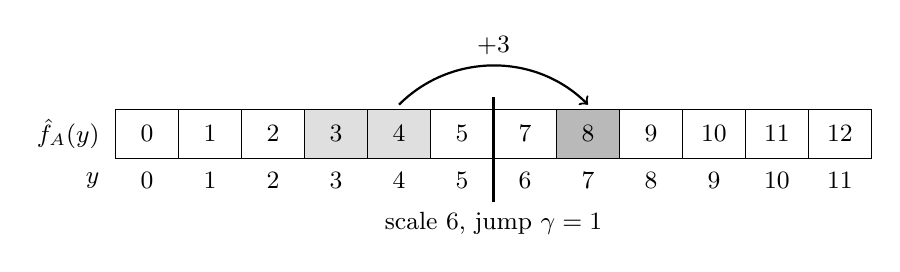
\begin{tikzpicture}[x=0.8cm,y=0.62cm,font=\small]
  \foreach \y in {3,4} \fill[gray!25] (\y,0) rectangle ++(1,1);
  \fill[gray!55] (7,0) rectangle ++(1,1);
  \foreach \y/\v in {0/0,1/1,2/2,3/3,4/4,5/5,6/7,7/8,8/9,9/10,10/11,11/12} {
    \draw (\y,0) rectangle ++(1,1);
    \node at (\y+0.5,0.5) {\v};
    \node at (\y+0.5,-0.45) {\y};
  }
  \node[anchor=east] at (-0.1,0.5) {$\ext A(y)$};
  \node[anchor=east] at (-0.1,-0.45) {$y$};
  \draw[very thick] (6,-0.9) -- (6,1.25);
  \node[anchor=north] at (6,-0.9) {scale $6$, jump $\jump=1$};
  \draw[->,thick] (4.5,1.1) to[bend left=45] node[above,midway] {$+3$} (7.5,1.1);
\end{tikzpicture}
\caption{The carry in \cref{ex:shah}. $A=(6,2):(1,7)$ adds $1$ to every offset beyond the scale
$6$. The two modes of $B$ contribute $4$ and $3$; their sum $7$ lies across the scale, so
$\ext A(7)=8=\ext A(4)+\ext A(3)+\jump$. A rule that composes the modes separately does not see
the carry.}\label{fig:carry}
\end{figure}

\noindent The published conditions for distributing over the modes of $B$ are sufficient
conditions of differing strength. The documentation~\cite{cutedocs} states that composition
distributes when $B$ is injective; \cref{ex:shah} shows that this is false. Cecka~\cite{cecka2026}
requires stride divisibility for every mode and that the modes be \emph{mutually segregated},
$t_ir_i\le r_j$ or $t_jr_j\le r_i$ for all $i\neq j$. If stride divisibility is demanded with
respect to all scales of $A$, this excluded interference in all our tests, and it is far from
necessary (for the $A$ above, $A\circ(2,2):(1,1)=(2,2):(1,1)$ although the two modes coincide).
If each mode is tested only against the scales that it reaches by itself, as in the single-mode
rule, the condition is not sufficient: for $A=(5,2):(1,6)$ and $B=(2,2):(2,4)$ the modes are
segregated and neither reaches the scale $5$, but $\ext A(2+4)=7\neq2+4$.
Shah~\cite[Def.~2.17, Thm.~2.18]{shah2024} requires that the \emph{intervals of definition}
$[r_j,(t_j-1)r_j]\cap[1,P_{m-1})$ of the modes be pairwise disjoint. That condition looks at two
modes at a time, and for three or more modes it is, as printed, not sufficient:

\begin{example}[three modes]\label{ex:three}
$A=(12,2):(1,13)$, $B=(2,2,2):(3,4,6)$. Every mode is admissible in the sense
of~\cite{shah2024}, and the intervals of definition are the single points $3$, $4$ and $6$. No
two of the three strides produce a carry across the scale $12$, but $3+4+6=13$ does:
$\ext A(13)=14$, whereas the concatenation of the per-mode composites, $(2,2,2):(3,4,6)$, gives
$13$.
\end{example}

\noindent The inequality of \cref{def:carryfree} involves all modes at once, and by
\cref{thm:carryfree} it is the exact condition for independent jumps: the modes of $B$ that land
on the same digit of $A$ must fit side by side inside that digit.

\paragraph{Incompleteness: non-monomial strides and non-dividing factors.}
For $t\ge2$ the rule produces only strides of the form $c\cdot d_k$. A composite may need more.

\begin{example}[sum strides]\label{ex:sumstride}
Let $A=\lay{(10,10,10)}{(d_0,d_1,d_2)}$ and $B=10:11$. The digit vector of $11$ is $(1,1,0)$ and
$9\cdot(1,1,0)$ causes no carry, so by \cref{cor:universal} $A\circ B=\lay{10}{(d_0+d_1)}$ for
every choice of strides; but $11$ neither divides nor is divisible by $10$, and the rule rejects
the pair. Similarly $\lay{(11,s)}{(d_0,d_1)}\circ 8:3=\lay{(4,2)}{(3d_0,\;d_0+d_1)}$ for all
$d_0,d_1$ and all $s\ge 2$: the refinement $(4,2):(3,12)$ of $8:3$ has stride digits $(3,0)$ and
$(1,1)$, and $3\cdot(3,0)+1\cdot(1,1)=(10,1)$ does not overflow the digit of size $11$.
\end{example}

The second example shows that even the single-term question ``when is $x\mapsto\floor{rx/P}$ a
layout function on $\rng t$?'' has a non-obvious answer; it is recorded in \cref{prop:dilated}.

\begin{proposition}[one dilated floor term]\label{prop:dilated}
Let $1\le\rho<q$ be coprime, $u=\ceil{q/\rho}$ and $e=u\rho-q$. The function
$x\mapsto\floor{\rho x/q}$ on $\rng t$ is a layout function if and only if $t\le u$, or $u\mid t$
and either $e=0$ or $t\le(\ceil{\rho/e}-1)\,u$. In the second case it equals $x\mapsto\floor{x/u}$.
\end{proposition}
\begin{proof}
The function is $0$ on $\rng u$ and increases by one at the points
$n_j=\ceil{jq/\rho}=ju-\floor{je/\rho}$, $j\ge1$. If $t\le u$ it vanishes. If $e=0$ then
$\rho\mid q$, so $\rho=1$, and the function is $x\mapsto\floor{x/u}$, a layout function on
$\rng t$ iff $u\mid t$ (\cref{thm:spectrum}(a)). Let $e\ge1$ and $J=\ceil{\rho/e}$. Since
$e<\rho$ we have $(J-1)e<\rho\le Je<2\rho$, so $n_j=ju$ for $j<J$ and $n_J=Ju-1$: the function
agrees with $\floor{x/u}$ below $Ju-1$ and exceeds it by $1$ there. Hence for $u<t\le Ju-1$ it
is a layout function iff $u\mid t$, i.e.\ iff $t\in\{2u,\dots,(J-1)u\}$; and for $t\ge Ju$ its
floor spectrum contains $u$ and $Ju-1$, which is not a multiple of $u$, so by
\cref{thm:spectrum}(a) it is not a layout function.
\end{proof}

\subsection{Laws}\label{sec:laws}

\begin{proposition}\label{prop:laws}
\begin{enumerate}[label=(\alph*),itemsep=1pt]
\item \emph{Identity.} $A\circ(\lay N1)$ is $A$ truncated or extended to size $N$, when that is
 a layout; and $(\lay N1)\circ B=B$.
\item \emph{Reshape.} For a column-major $B$ with shape $T$ (so $\bnd B$ is the identity),
 $A\circ B$ exists if and only if $\spec(\ext A|_{\rng{|T|}})\cup\Sc(T)\cup\{|T|\}$ is a chain
 under divisibility.
\item \emph{Distributivity.} $A\circ(B_0,\dots,B_{n-1})=(A\circ B_0,\dots,A\circ B_{n-1})$ holds
 exactly when the right-hand side exists and the non-interference condition of
 \cref{thm:exact}(iii) is satisfied.
\item \emph{Associativity.} Let $C$ be $\N$-valued with $\bnd C(\rng{|C|})\subseteq\rng{|B|}$, and
 suppose $A\circ B$ and $B\circ C$ exist, $B\circ C$ being represented as in \cref{thm:exact}
 (each $R_j$ coalesced). If $(A\circ B)\circ C$ and $A\circ(B\circ C)$ both
 exist, they have the same function. If $A\circ(B\circ C)$ exists then so does
 $(A\circ B)\circ C$. The converse can fail.
\item \emph{Additivity in $A$.} If $A_1,A_2$ have the same shape then
 $(A_1+A_2)\circ B=A_1\circ B+A_2\circ B$ over any refinement over which both sides exist.
\end{enumerate}
\end{proposition}
\begin{proof}
(a) and (e) are immediate. (b) is \cref{thm:exact}(iv) with $g=\ext A|_{\rng{|T|}}$: the set is
a chain iff $g$ is a layout function (\cref{thm:spectrum}(a)) whose spectrum is compatible with
$\Sc(T)$. (c) is \cref{thm:exact}. (d): by the in-bounds hypothesis the extended function of the
layout $A\circ B$ agrees with $\ext A\circ\bnd B$ on the values of $C$, so each bracketing, if it
exists, represents $h=\ext A\circ\bnd B\circ\bnd C$. By \cref{thm:exact}, $(A\circ B)\circ C$
exists iff $h$ is additive over a by-mode refinement of the shape of $C$, whereas
$A\circ(B\circ C)$ exists iff $h$ is additive over a by-mode refinement of the shape of the
layout $B\circ C$, which itself refines the shape of $C$. This gives the implication, and shows
why the converse may fail: the intermediate layout $B\circ C$ may have scales that $h$ does not
tolerate. (The representative matters: for $A=(2,3):(0,1)$ and $B=C=6:1$, composing $A$ with
$B\circ C=6:1$ works, whereas the finer layout $(3,2):(1,3)$ with the same function would not
do.)
\end{proof}

\begin{example}[associativity]\label{ex:assoc}
Let $A=(12,3):(0,1)$, $B=(2,2,3,3):(1,6,2,12)$ and $C=6:7$; the values of $C$ lie in
$\rng{36}=\rng{|B|}$. Here $\bnd B$ permutes each block of $12$ consecutive numbers, so
$A\circ B$ has function $\floor{x/12}$, and $(A\circ B)\circ C=(2,3):(0,1)$ with function
$h(x)=\floor{7x/12}=\floor{x/2}$ on $\rng6$. But $B\circ C=(3,2):(9,17)$ has the scale $3$,
which is incomparable with the scale $2$ of $h$, so $A\circ(B\circ C)$ does not exist. Without
the in-bounds hypothesis even the functions can differ~\cite{cecka2026}:
$\bigl((5,3):(1,7)\circ4:1\bigr)\circ2:5=2:5$ but $(5,3):(1,7)\circ\bigl(4:1\circ2:5\bigr)=2:7$.
\end{example}

\section{Complement, division and product}\label{sec:complement}

In this section layouts are $\N$-valued unless stated otherwise, and the \emph{image} of a layout
$A$ is the set $\bnd A(\rng{|A|})\subseteq\N$.

\subsection{Complements are direct-sum decompositions of an interval}

CuTe's complement is meant to describe ``the elements not touched by $A$'' as the layout of the
\emph{repetitions} of $A$. The clean way to say this is with sumsets.

\begin{definition}\label{def:directsum}
For $I,J\subseteq\N$ and $M\ge1$ we write $I\oplus J=\rng M$ if $(a,b)\mapsto a+b$ is a bijection
$I\times J\to\rng M$. A layout $C$ is a \emph{complement of $A$ in $\rng M$} if the concatenated
layout $(A,C)$ is a bijection onto $\rng M$; equivalently, $\bnd A$ and $\bnd C$ are injective and
their images $I,J$ satisfy $I\oplus J=\rng M$.
\end{definition}

Pairs $(I,J)$ with $I\oplus J=\rng M$ are a classical subject, known as Krasner factorisations
(see~\cite{bodini2006}). De~Bruijn~\cite{debruijn1956} determined the pairs with $I\oplus J=\N$;
for the finite case we use the formulation of Long~\cite{long1967}:

\begin{theorem}[Long {\cite[Thm.~1]{long1967}}]\label{thm:long}
Let $M\ge2$. Sets $I,J\subseteq\N$ satisfy $I\oplus J=\rng M$ if and only if there are integers
$m_1,\dots,m_r\ge2$ with $m_1\cdots m_r=M$ such that, with $M_k=m_1\cdots m_k$, one of the two
sets consists of all sums $\sum_{k\text{ even}}x_kM_k$ and the other of all sums
$\sum_{k\text{ odd}}x_kM_k$, where $0\le x_k<m_{k+1}$ and $0\le k<r$.
\end{theorem}

\noindent In words: the direct-sum decompositions of an interval are exactly the splittings of the
digits of some mixed-radix system into the even and the odd positions. Both summands are
therefore images of layouts, and CuTe's formula for the complement---interleave the modes of $A$,
sorted by stride, with the modes that fill the gaps---is the only thing a complement can be. The
complement is moreover unique as a set, as noted by Bodini and Rivals~\cite[\S3]{bodini2006}; we
include the short argument.

\begin{proposition}[uniqueness {\cite{bodini2006}}]\label{prop:unique-complement}
For $I\subseteq\N$ and $M\ge1$ there is at most one $J\subseteq\N$ with $I\oplus J=\rng M$.
\end{proposition}
\begin{proof}
Let $J\neq J'$ both qualify; then $0\in I\cap J\cap J'$. Let $z$ be the least element in which
$J$ and $J'$ differ, say $z\in J\setminus J'$. Since $z=0+z\in\rng M=I\oplus J'$, we have $z=a+b'$
with $a\in I$, $b'\in J'$; as $z\notin J'$, $a>0$ and $b'<z$, so $b'\in J$. Then $z=0+z=a+b'$
are two representations in $I+J$, a contradiction.
\end{proof}

\begin{theorem}[complement]\label{thm:complement}
Let $A$ be an $\N$-valued layout with injective function and image $I$, with at least one non-unit
mode, and let $M\ge1$. Let $(d_{(0)},s_{(0)}),\dots,(d_{(k)},s_{(k)})$ be the strides and sizes of
its non-unit modes, sorted by stride. The following are equivalent:
\begin{enumerate}[label=(\roman*),itemsep=1pt]
\item there is a set $J$ with $I\oplus J=\rng M$;
\item $A$ has a complement in $\rng M$;
\item $s_{(i)}d_{(i)}\mid d_{(i+1)}$ for $0\le i<k$, and $s_{(k)}d_{(k)}\mid M$.
\end{enumerate}
In that case $J$ is the image of
\begin{equation}\label{eq:complement}
 C=\lay{\Bigl(d_{(0)},\ \frac{d_{(1)}}{s_{(0)}d_{(0)}},\ \dots,\ \frac{d_{(k)}}{s_{(k-1)}d_{(k-1)}},\ \frac{M}{s_{(k)}d_{(k)}}\Bigr)}{\bigl(1,\ s_{(0)}d_{(0)},\ \dots,\ s_{(k)}d_{(k)}\bigr)},
\end{equation}
$\bnd C$ is increasing, and $\coal(C)$ is the only coalesced layout with increasing function that
is a complement of $A$ in $\rng M$. {\rm(}If all modes of $A$ are unit modes then $I=\{0\}$ and the
complement is $\lay M1$.{\rm)}
\end{theorem}
\begin{proof}
Injectivity gives $d_{(0)}\ge1$.
(iii)$\Rightarrow$(ii): sorting the modes of $(A,C)$ by stride gives the column-major layout with
shape $(d_{(0)},s_{(0)},d_{(1)}/(s_{(0)}d_{(0)}),s_{(1)},\dots)$, a bijection onto
$\rng M$~\cite[Prop.~2.7]{shah2024}. (ii)$\Rightarrow$(i) is trivial, and (i)$\Rightarrow$(ii)
holds because $J$ is the image of a layout by \cref{thm:long}.
(ii)$\Rightarrow$(iii): let $E=(A,C')$ be a bijection onto $\rng M$ and let
$(r_{(0)},t_{(0)}),(r_{(1)},t_{(1)}),\dots$ be its non-unit modes sorted by stride. We claim
$r_{(j)}=\Pi_j:=t_{(0)}\cdots t_{(j-1)}$. Inductively, the coordinates supported on the modes
$(0),\dots,(j-1)$ take exactly the values in $\rng{\Pi_j}$. The unit of mode $(j)$ is a different
coordinate, so by injectivity $r_{(j)}\ge\Pi_j$; and the value $\Pi_j$ is attained by a coordinate
with a non-zero entry in some mode $(j')$, $j'\ge j$, so $\Pi_j\ge r_{(j')}\ge r_{(j)}$. Thus the
sorted layout is column-major, and the modes of $A$ occur in it in the order of their strides, so
$s_{(i)}d_{(i)}$, a prefix product, divides the later prefix product $d_{(i+1)}$, and
$s_{(k)}d_{(k)}$ divides $M$. (This direction is \cite[Prop.~2.1.6.32]{carlisle2026}.)
Finally, $J$ is unique by \cref{prop:unique-complement}, an increasing function is determined by
its image, and a coalesced layout by its function (\cref{cor:coalesce}); $\bnd C$ is increasing
because each stride of $C$ exceeds the largest value reachable with the earlier modes.
\end{proof}

The equivalence of (ii) and (iii) and the uniqueness of the sorted coalesced complement are due
to Shah~\cite{shah2024} and Carlisle et al.~\cite{carlisle2026}. What \cref{thm:long} adds is
that condition (iii) is not a restriction imposed by the layout formalism: \emph{no set
whatsoever} completes $I$ to an interval unless (iii) holds. Uniqueness of the set $J$ gives an
involution for free (again noted for sets in~\cite{bodini2006}):

\begin{corollary}[double complement]\label{cor:double}
If $A$ has a complement $C$ in $\rng M$, then the complement of $C$ in $\rng M$ is the
coalesced, increasing layout with the same image as $A$ (``sort the modes of $A$ by stride and
coalesce'').
\end{corollary}
\begin{proof}
Both have image the unique $I'$ with $I'\oplus J=\rng M$, namely $I$, and increasing functions.
\end{proof}

\begin{remark}[beyond the tiling regime]\label{rem:nontiling}
CuTe's \code{complement} is defined more generally. If only the last clause of (iii) fails and
the cotarget is an integer $M$, the implementations round $M$ up to the next multiple $M'$ of
$s_{(k)}d_{(k)}$ and return the complement in $\rng{M'}$; this is how tiles that overhang the end of a tensor arise. If the
chain condition itself fails but $s_{(i)}d_{(i)}\le d_{(i+1)}$ still holds, they replace the
quotients in~\eqref{eq:complement} by their integer parts. The result $C$ then has an increasing
function and $(A,C)$ is injective, but it is not onto any interval, and by \cref{thm:complement}
no set could make it so. The stated post-conditions (disjoint, ordered) do not determine $C$ in
this regime---for $A=(2,2):(1,3)$ and $M=24$ both $4:6$, which is returned, and $4:5$ satisfy
them---and we do not study it.
\end{remark}

\subsection{Compact layouts and division}

A layout $E$ is \emph{compact} if $\bnd E$ is a bijection onto $\rng{|E|}$. The proof of
\cref{thm:complement} showed (cf.~\cite[Prop.~2.1.5.6]{carlisle2026}, \cite[\S3]{shah2024}):

\begin{lemma}[compact layouts are digit permutations]\label{lem:compact}
A flat layout $E=\lay TR$ is compact if and only if its non-unit modes, sorted by stride, form a
column-major layout $U$. Then $\bnd E$ sends the digit $c_j$ of mode $j$ of $T$ to the digit of
$U$ at the position that mode $j$ takes in the sorted order.
\end{lemma}
\noindent We call $U$ the \emph{sorted shape} of $E$. Thread-value layouts of tensor-core
instructions and the layouts $(B,\compl(B,M))$ that implement tiling are compact.

\begin{theorem}[composition with a compact layout]\label{thm:division}
Let $E$ be a compact layout of size $M$ with sorted shape $U$, and let $A$ be a layout with values
in any abelian group $\D$. Then $A\circ E$ exists if and only if
\[ \spec(\ext A|_{\rng M})\ \cup\ \Sc(U)\ \cup\ \{M\}\quad\text{is a chain under divisibility,} \]
that is, if and only if $\ext A|_{\rng M}$ is a layout function whose spectral scales are
comparable with the scales of $U$. If $|A|=M$ the first requirement holds automatically.
\end{theorem}
\begin{proof}
Let $T'$ be a by-mode refinement of the shape $T$ of $E$, and $E'$ the corresponding refinement of
$E$. $E'$ is compact; its sorted shape $U'$ refines $U$, and conversely every refinement of $U$
arises this way (subdivide a mode of $T$ exactly as the corresponding digit of $U$). By
\cref{lem:compact}, $\bnd E=\bnd{E'}$ carries the digits of $T'$ to those of $U'$, hence
carry-free pairs for $T'$ to carry-free pairs for $U'$, and vice versa. So $\ext A\circ\bnd E$ is
$T'$-additive iff $\ext A|_{\rng M}$ is $U'$-additive, iff
$\spec(\ext A|_{\rng M})\subseteq\Sc(U')$ (\cref{thm:spectrum}). The sets $\Sc(U')$, for $U'$
refining $U$, are the chains of divisors of $M$ in $\{2,\dots,M-1\}$ that contain $\Sc(U)$; one
of them contains the spectrum iff the displayed set is a chain. The last sentence is
\cref{thm:spectrum}(a).
\end{proof}

\begin{corollary}[logical divide]\label{cor:divide}
Let $A$ be any layout and let $B$ have a complement in $\rng{|A|}$. Then
$A\oslash B=A\circ(B,\compl(B,|A|))$ exists if and only if every spectral scale of $\bnd A$ is
comparable under divisibility with each of the numbers $d_{(i)}$ and $s_{(i)}d_{(i)}$ attached to
$B$ in \cref{thm:complement}.
\end{corollary}
\begin{proof}
The prefix products of the sorted shape of $(B,\compl(B,|A|))$ are
$1$, $d_{(0)}$, $s_{(0)}d_{(0)}$, $d_{(1)}$, \dots, $s_{(k)}d_{(k)}$, $|A|$.
\end{proof}

\begin{example}
Tile $A=(8,8):(1,9)$, a padded $8\times8$ matrix with the single spectral scale $8$, by $B=4:1$:
here $\compl(B,64)=16:4$ and the tiling has the scale $4$, which divides $8$. So
$A\oslash B$ exists; it is $(4,(2,8)):(1,(4,9))$. For $A=(6,8):(1,7)$ and the same $B$ the scales
$4$ and $6$ are incomparable: $A\oslash B$ does not exist, for any choice of strides with a
non-zero jump at $6$.
\end{example}

\begin{remark}[tilers that do not divide the size]\label{rem:roundup}
When $s_{(k)}d_{(k)}\nmid|A|$, $B$ has no complement in $\rng{|A|}$ and \cref{cor:divide} does not
apply. If one divides by the complement of $B$ in the longer interval $\rng{M'}$ of
\cref{rem:nontiling} instead, $A$ is evaluated beyond its domain and \cref{thm:division} applies
with $M'$ in place of $M$; its requirement that the spectral scales divide $M'$ is then a real
one. For $A=(2,2):(0,1)$ and $B=5:1$ one has $M'=5$ and a tiling without proper scales, but
$\ext A(x)=\floor{x/2}$ is not a layout function on $\rng5$, and the composite does not exist.
The implementations pass a shape rather than an integer as the cotarget in \code{logical\_divide}
and need not follow this recipe: in PyCuTe, dividing $(2,2):(1,2)$ by $3:1$ returns
$(3,1):(1,3)$, a layout of size $3$.
\end{remark}

\Cref{thm:division} is exact and makes no assumption on $A$. When $A$ is itself a digit map it
specialises to the ``mutual refinement'' criterion of Carlisle et al.~\cite[\S4.1]{carlisle2026},
who also sketch, without proof, the extension to a general outer layout using rational
entries~\cite[\S4.1.5]{carlisle2026}; for a compact inner layout the theorem makes that precise
and supplies the converse.

It also shows how compact layouts compose, and why care is needed. A compact layout $E$ comes
with two chains: the spectrum of $\bnd E$, on the side of its domain, and $\Sc(U)$, on the side
of its codomain. By \cref{thm:division}, for compact layouts $E_1,E_2$ of the same size,
$E_1\circ E_2$ exists if and only if the domain chain of $E_1$ is compatible with the codomain
chain of $E_2$. It is not enough that the two sorted shapes
have a common refinement: $E=(2,3):(3,1)$ has sorted shape $(3,2)$, but $E\circ E$ would be the
permutation $(0,4,3,2,1,5)$, which is not a layout function. So the permutations of $\rng M$
expressible as layouts do not form a group; as observed in~\cite[\S3]{shah2024} they are the image
of a groupoid whose objects are the ordered factorisations of $M$, a compact layout being a
morphism from its domain chain to its codomain chain.

\subsection{Product and inverses}

For completeness we record how the remaining operations fit in.

\begin{proposition}\label{prop:product}
\begin{enumerate}[label=(\alph*),itemsep=1pt]
\item Let $A$ be injective with at least one non-unit mode, let it satisfy condition (iii) of
 \cref{thm:complement} without the last clause, and let $A^*$ be the layout~\eqref{eq:complement}
 with last mode $\lay1{s_{(k)}d_{(k)}}$. Then $(a,b)\mapsto a+b$ is a bijection from
 $I\times\ext{A^*}(\N)$ onto $\N$, all jumps of $A^*$ are positive, and the logical product
 $A\otimes B=(A,A^*\circ B)$ exists if and only if some by-mode refinement of $B$ is carry-free at
 the scales of $A^*$. It is injective iff $B$ is.
\item If $E$ is compact with sorted shape $U$, then $\bnd E^{-1}$ is the function of the compact
 layout with shape $U$ whose strides are the prefix products of the shape of $E$, taken in sorted
 order. More generally, if some of the modes of a layout $A$, sorted by stride, form a
 column-major layout of size $K$, then the inverse of that sublayout, read as a map into the
 domain of $A$, is a right inverse of $A$ on $\rng K$. If $A$ has a complement in $\rng M$, the
 inverse of $(A,\compl(A,M))$ is a left inverse of $A$, i.e.\ it sends $\bnd A(x)$ to $x$.
\end{enumerate}
\end{proposition}
\begin{proof}
(a) The bijection follows from \cref{thm:complement} applied to all multiples $M$ of
$s_{(k)}d_{(k)}$. The jumps of $A^*$ are $(s_{(i)}-1)\,d_{(i)}>0$, hence independent, and
\cref{thm:carryfree} applies. (b) By \cref{lem:compact}, $\bnd E$ permutes mixed-radix digits; the
inverse permutation has the stated strides. The other two statements follow by restricting to
the coordinates of the chosen modes, respectively of $A$.
\end{proof}

\noindent CuTe's \code{right\_inverse} selects such a set of modes greedily in order of
increasing stride; the result is a right inverse but not always the largest one (for
$A=(2,3):(1,1)$ the greedy choice has size $2$, while $3:2$ is a right inverse of size $3$).
Its \code{left\_inverse} may differ from the inverse of $(A,\compl(A,M))$ outside the image of
$A$, where a left inverse is unconstrained.

\section{Other codomains, and the categorical picture}\label{sec:beyond}

\subsection{Negative strides, coordinates, XOR}

Nothing in \cref{sec:carry,sec:normalform,sec:composition} used more about the codomain $\D$ of
the outer layout than that it is an abelian group. Three instances matter in practice.

\emph{$\D=\Z$ with negative strides} (reversed modes). The inner layout $B$ of a composition
must still be $\N$-valued, since it produces arguments of $\ext A$.

\emph{$\D=\Z^k$: coordinate layouts.} Cecka~\cite{cecka2026} uses strides that are multiples of
basis vectors $e_i$ to make layouts return coordinates rather than offsets; e.g.\
$(4,8):(e_0,e_1)$ is the identity on $2$-D coordinates. The digit layout $E_S$ of
\cref{sec:composition} is of this kind, and \cref{cor:universal} says that it is the universal
outer layout: $A\circ B$ exists for all strides on $S$ exactly when $E_S\circ B$ does.

\emph{$\D=\F_2^k$: XOR.} Let $S=(2,\dots,2)$ have $m$ binary modes. A layout
$\lay SD$ with $D\in(\F_2^k)^m$ sends $x$ to the XOR of the strides $d_i$ over the set bits $i$ of
$x$: it is an arbitrary $\F_2$-linear map $\F_2^m\to\F_2^k$ precomposed with the binary expansion.
These are precisely the \emph{linear layouts} of Triton~\cite{zhou2026}, and they include the
swizzle patterns used to avoid shared-memory bank conflicts.\footnote{PyCuTe's \code{F2} strides
multiply carry-lessly, which amounts to reading a mode of size $2^p$ as $p$ binary modes; with
that reading its XOR-strided layouts are of this form. Beyond its last mode PyCuTe continues
carry-lessly, with further binary modes of strides $2^pd,2^{p+1}d,\dots$, whereas
\cref{def:layout} would let the coordinate of the last mode grow.} Since $2d=0$ in $\F_2^k$, the jumps of
such a layout are its strides, $\jump_i=d_i$, and the carry identity reads
\[ \ext L(x+y)=\ext L(x)\oplus\ext L(y)\oplus\bigoplus_{i\ge1}c_i(x,y)\,d_i , \]
which for the identity layout, and $x+y<2^m$, is the textbook equation of the binary adder.
\Cref{thm:defect} applies unchanged: such a layout $A$ composes with an $\N$-valued $B$ as
long as the carries of $B$ in binary are invisible to $A$, e.g.\ when the modes of $B$ occupy
disjoint bit ranges, as the modes of a compact layout with power-of-two mode sizes do
(thread-value layouts of tensor-core instructions are of this kind). \Cref{sec:swizzle} works
this out for CuTe's swizzles.

This also explains a difference that is often noted between the two systems: composition of
Triton's linear layouts is total, while CuTe's is partial. In Triton the intermediate object is a
bit vector and intermediate values are combined by XOR, the carry-less addition of
\cref{rem:twogroups}; no carries arise and the composite of linear maps is linear. In CuTe the
intermediate object is an integer offset, intermediate values are combined by integer addition,
and the composite is a layout exactly when the resulting carries cancel (\cref{thm:exact}). The
price Triton pays is the restriction to shapes that are powers of two, where the two additions
can be told apart bit by bit.

\subsection{Boxes and lifting}\label{sec:box}

The results can be organised categorically; this subsection is not needed elsewhere. We
consider shapes without unit modes (unit modes carry no information about functions). For such a
shape $S$ let $\BoxC(S)=\rng{s_0}\times\dots\times\rng{s_{m-1}}\subseteq\N^m$, with the partial addition
that is defined on carry-free pairs. A \emph{morphism} $S\to T$ is a map
$\BoxC(S)\to\BoxC(T)$ that preserves this partial addition; equivalently, a matrix
$\Phi\in\N^{n\times m}$ with $\Phi\,(s_i-1)_i\le(t_j-1)_j$ componentwise. Morphisms compose by
matrix multiplication, and by \cref{prop:additive} a layout on $S$ with values in $\D$ is the
same thing as an additive map $\BoxC(S)\to\D$, given by the row vector of strides.

In this category the colexicographic bijection $\kappa_S\colon\BoxC(S)\to\BoxC((|S|))=\rng{|S|}$,
with matrix $(P_0,\dots,P_{m-1})$, is a morphism, and so is every coarsening map between
compatible shapes; but their inverses---digit expansion---are not, as soon as two modes are
merged. \emph{This is the whole source of partiality.} An $\N$-valued layout $B$ on $T$ with values below $M$ is a morphism
$T\to(M)$; to compose it with a layout $A$ on a shape $S$ of size $M$ one must first \emph{lift} it
along $\kappa_S$:
\[
 \BoxC(T')\xrightarrow{\ \Phi\ }\BoxC(S)\xrightarrow{\ D\ }\D,
 \qquad \kappa_S\circ\Phi=B\circ\kappa_{T'\to T},
\]
for some by-mode refinement $T'$ of $T$. For a given $T'$ the lift is unique if it exists---its
columns are the digit vectors of the strides of $B'$---and it exists exactly when $B'$ is
carry-free at all scales of $S$; then $A\circ B=D\Phi$. That is \cref{cor:universal}. When no lift exists a particular $A$
may still compose with $B$, namely when its jumps annihilate the carries (\cref{thm:exact}).

Up to the bookkeeping of unit entries, the category $\mathsf{Tuple}$ of Carlisle et
al.~\cite{carlisle2026} is the subcategory whose morphisms are the matrices with columns $0$ or
$e_j$ (distinct for distinct columns) and matching sizes $s_i=t_j$; their \emph{tractable} layouts are the composites $\kappa_T\circ\Phi$ of such
morphisms with a colexicographic map, and their ``mutual refinement'' is the lifting condition in
that case. The present framework removes the restriction to tractable layouts at the cost of
replacing diagrams by one inequality.

\section{Swizzles}\label{sec:swizzle}

Shared-memory layouts in CUTLASS kernels are \emph{swizzled}: offsets are permuted by an XOR
pattern so that the accesses of a warp fall into distinct memory banks. C++ CuTe models this by a
function object \code{Swizzle<B,M,S>} and by \code{ComposedLayout}, a triple (swizzle, offset,
layout) that stands for the function $c\mapsto\sigma(o+f(c))$~\cite{cutedocs}; PyCuTe instead
gives layouts strides in $\F_2$~\cite{cecka2026,pycute}. Apart from the identity, a swizzle is not
additive for integer addition, so a swizzled layout is in general not a layout in the sense of
\cref{sec:background}. This section shows
that swizzles nevertheless belong to the carry calculus. Offsets carry two group laws, integer
addition and bitwise XOR; a swizzle is a layout for the second; and the two laws differ exactly
by the carries of the binary radix, which \cref{thm:carry} keeps account of.

\subsection{A swizzle is a layout for XOR}

For $x\in\N$ let $\bit_b(x)\in\{0,1\}$ be its $b$-th binary digit and
$\operatorname{supp}(x)=\{b:\bit_b(x)=1\}$; $\oplus$ is bitwise XOR. Let
$\beta\colon\N\to\F_2^{(\N)}=\bigoplus_b\F_2e_b$, $\beta(x)=\sum_b\bit_b(x)\,e_b$, be the binary
expansion; it is a bijection that turns $\oplus$ into addition. By \cref{def:layout}, $\beta$ is
the function of the layout $\lay{(2,2,\dots)}{(e_0,e_1,\dots)}$ with values in $\F_2^{(\N)}$
(with $k$ modes for offsets below $2^k$). Its jumps are $e_b-2e_{b-1}=e_b$ at the scales $2^b$,
$b\ge1$, and \cref{thm:carry} for this layout is the equation of the binary adder,
\begin{equation}\label{eq:adder}
 \beta(x+y)=\beta(x)+\beta(y)+\sum_{b\ge1}c_b(x,y)\,e_b,
 \qquad\text{i.e.}\qquad x+y=x\oplus y\oplus(\text{carry word}).
\end{equation}

\begin{definition}[swizzle]\label{def:swizzle}
A \emph{pairing} $\pi$ is a finite set of pairs $(y\to z)$ of bit positions in which no position
occurs twice. Its \emph{swizzle} $\sigma_\pi\colon\N\to\N$ replaces, for every pair, bit $z$ by
$\bit_z\oplus\bit_y$:
\[ \sigma_\pi(x)=x\oplus\bigoplus_{(y\to z)\in\pi}\bit_y(x)\,2^z . \]
CuTe's \code{Swizzle<B,M,S>}, with $B,M\ge0$ and $|S|\ge B$, is the pairing
$\{(M+S+i\to M+i):i<B\}$ if $S>0$ and $\{(M+i\to M+|S|+i):i<B\}$ if $S<0$: a field $Y$ of $B$
consecutive bits is XOR-ed into a field $Z$ at distance $|S|$ (``\code{ZZZ \^{}= YYY}''); for $B=0$
the pairing is empty and the swizzle is the identity. We put $T=M+B+|S|$, the first bit position
above both fields.
\end{definition}

\noindent The C++ functor keeps its two masks as $32$-bit signed integers. It computes $\sigma_\pi$
as long as both fields lie within bits $0$--$30$, which we assume when we speak of CuTe's swizzles;
a field that reaches bit $31$ is sign-extended against a $64$-bit offset, and then, for instance,
\code{Swizzle<1,30,1>} is no longer an involution.

\begin{example}[the 128-byte swizzle]\label{ex:sw128}
\code{Swizzle<3,4,3>} acts on byte addresses. A block of $1024$ bytes is seen as $8$ rows of
$128$ bytes, each row as $8$ chunks of $16$ bytes; the chunk index $z$ (bits $4$--$6$) is replaced
by $z\oplus y$, where $y$ (bits $7$--$9$) is the row index. For fixed $y$ the map $z\mapsto z\oplus y$
permutes the chunks of a row, so each row still occupies its own $128$ bytes; for fixed $z$ the map
$y\mapsto z\oplus y$ is a bijection as well. In other words $(y,z)\mapsto z\oplus y$ is a Latin
square: a column of the tile, which without the swizzle sits at the same chunk position in every
row (and so, when the row length is a multiple of the bank period, in the same banks), is spread
over all $8$ chunk positions (\cref{fig:swizzle}).
\end{example}

\begin{figure}[t]\centering
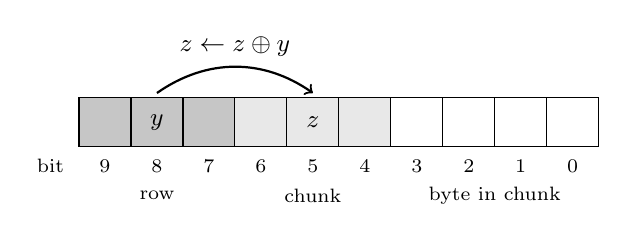
\begin{tikzpicture}[x=0.66cm,y=0.62cm,font=\small,baseline=(current bounding box.center)]
  \fill[gray!45] (0,0) rectangle (3,1);
  \fill[gray!18] (3,0) rectangle (6,1);
  \foreach \b in {0,...,9} {
    \draw (9-\b,0) rectangle ++(1,1);
    \node[font=\scriptsize] at (9.5-\b,-0.4) {\b};
  }
  \node at (1.5,0.5) {$y$};
  \node at (4.5,0.5) {$z$};
  \node[font=\scriptsize] at (1.5,-1.0) {row};
  \node[font=\scriptsize] at (4.5,-1.0) {chunk};
  \node[font=\scriptsize] at (8,-1.0) {byte in chunk};
  \node[anchor=east,font=\scriptsize] at (-0.1,-0.4) {bit};
  \draw[->,thick] (1.5,1.1) to[bend left=35] node[above,midway] {$z\leftarrow z\oplus y$} (4.5,1.1);
\end{tikzpicture}
\qquad\qquad
$\begin{array}{c|cccc}
 y\backslash z&0&1&2&3\\\hline
 0&0&1&2&3\\ 1&1&0&3&2\\ 2&2&3&0&1\\ 3&3&2&1&0
\end{array}$
\caption{Left: the bit fields of a byte address under \code{Swizzle<3,4,3>} (\cref{ex:sw128}); the
field $Y$ (dark) is XOR-ed into the field $Z$ (light). Right: the chunk position $z\oplus y$ of
logical chunk $z$ in row $y$ for two-bit fields; every row and every column is a permutation.}
\label{fig:swizzle}
\end{figure}

\begin{lemma}[structure of a swizzle]\label{lem:swizzle}
Let $\sigma=\sigma_\pi$.
\begin{enumerate}[label=(\alph*),itemsep=1pt]
\item $\sigma$ is an involution of $\N$, and
 $\sigma(x)=x+\sum_{(y\to z)\in\pi}2^z\,\bit_y(x)\bigl(1-2\,\bit_z(x)\bigr)$.
\item $\sigma(x\oplus x')=\sigma(x)\oplus\sigma(x')$. Equivalently $\beta\circ\sigma=\Lambda\circ\beta$
 for the linear map $\Lambda=1+N$ with $Ne_y=e_z$ for $(y\to z)\in\pi$ and $Ne_b=0$ otherwise.
 Hence $\beta\circ\sigma$ is the function of the layout
 $\lay{(2,2,\dots)}{(\Lambda e_0,\Lambda e_1,\dots)}$ with values in $\F_2^{(\N)}$.
\item If all positions of $\pi$ are below $T$, then $\sigma(x+2^Tq)=\sigma(x)+2^Tq$ for $x<2^T$.
 If all are at least $M$, then $\sigma(x)\equiv x\pmod{2^M}$.
\item If $z<y$ for every pair (as for $S>0$), then $\sigma$ permutes $\rng{2^t}$ for every $t\ge0$.
\end{enumerate}
\end{lemma}
\begin{proof}
Only the bits $z$ change, and the bits $y$ do not; so applying $\sigma$ twice restores every bit.
For two bits, $(b\oplus a)-b=a(1-2b)$, which gives the formula. (b) holds because every bit of
$\sigma(x)$ is an $\F_2$-linear function of the bits of $x$. (c) and (d) are read off the
definition; for (d), if $x<2^t$ then the pairs with $y\ge t$ are inactive and those with $y<t$
change a bit below $t$.
\end{proof}

\noindent So a swizzle \emph{is} a layout, as soon as offsets are added by XOR. What makes
swizzled layouts delicate is that the layout underneath adds its contributions as integers.

\subsection{Swizzled layouts}

A \emph{swizzled layout} is a triple $(\sigma,o,f)$ of a swizzle, an offset $o\in\N$ and an
$\N$-valued layout $f=\lay TR$ with $T=(t_0,\dots,t_{n-1})$, $R=(r_0,\dots,r_{n-1})$; its function
is $h(c)=\sigma(o+f(c))$. It is the composite of the $\F_2$-valued layout of
\cref{lem:swizzle}(b) with an integer layout, so \cref{thm:defect} applies to it.

\begin{theorem}[composition formula for swizzled layouts]\label{thm:swzcomp}
For every $c\in\rng{t_0}\times\dots\times\rng{t_{n-1}}$,
\begin{align*}
 \sigma\Bigl(o+\sum_jc_jr_j\Bigr)&=\sigma(o)\;\oplus\bigoplus_{j\,:\,c_j\text{ odd}}\sigma(r_j)
 \;\oplus\bigoplus_{b\ge1\,:\,\Cdef_b(c)\text{ odd}}\sigma(2^b),\\
 \Cdef_b(c)&=\floor{\frac{(o\bmod2^b)+\sum_jc_j\,(r_j\bmod2^b)}{2^b}} .
\end{align*}
\end{theorem}
\begin{proof}
Let $A$ be the layout of \cref{lem:swizzle}(b), and let $B'$ be the inner layout with shape
$(2,t_0,\dots,t_{n-1})$ and strides $(o,r_0,\dots,r_{n-1})$. Apply \cref{thm:defect} to $A$ and
$B'$ at the coordinate $(1,c)$. The jump of $A$ at scale $2^b$ is
$\Lambda e_b=\beta(\sigma(2^b))$, and in $\F_2^{(\N)}$ a multiple $m\cdot v$ is $v$ or $0$
according to the parity of $m$.
\end{proof}

A swizzled layout is thus XOR-linear in the coordinates \emph{up to the parity of the binary
carries} that the inner layout produces. Two cases in which it reduces to a layout over a single
group can be described exactly.

\begin{definition}\label{def:bitdisjoint}
A layout $\lay TR$ with values in $\N$ is \emph{bit-disjoint} if every mode with non-zero stride
has a size that is a power of two, and the numbers $2^b\,r_j$ ($0\le b<\log_2t_j$, $r_j\ne0$)
have pairwise disjoint supports. Its \emph{binary refinement} replaces every mode of size
$t_j\ge2$ with $r_j\neq0$ by $\log_2t_j$ binary modes with these numbers as strides, and keeps the
unit modes and the modes with stride $0$ (giving them the stride $0$); if
$\rho_1,\dots,\rho_p$ are the strides of its binary modes and $c_1,\dots,c_p\in\{0,1\}$ their
coordinates, then $f(c)=\bigoplus_lc_l\rho_l$.
\end{definition}
\noindent Compact layouts with power-of-two mode sizes are bit-disjoint: they permute the binary
digits. So is every layout obtained from one by dropping modes, e.g.\ the tiles of a power-of-two
array.

\begin{corollary}[XOR-linear swizzled layouts]\label{cor:xorlinear}
For a swizzle $\sigma$, the map $c\mapsto\sigma(f(c))$ is the function of an $\F_2$-valued
layout over a by-mode refinement of $T$ if and only if $f$ is bit-disjoint. In that case it is the
layout over the binary refinement with the strides $\beta\sigma(\rho_1),\dots,\beta\sigma(\rho_p)$
on the binary modes and $0$ on the others.
\end{corollary}
\begin{proof}
If $f$ is bit-disjoint, no carries occur on the binary refinement and \cref{thm:swzcomp} gives
the claim. Conversely, in an $\F_2$-valued layout a mode of size at least $3$ with stride $v$
takes the value $2v=0$ at its coordinate $2$; as $\sigma$ is injective and $\sigma(0)=0$, such a
mode of the refinement has integer stride $0$. Hence every mode of $f$ with $r_j\neq0$ is refined
into binary modes, so $t_j$ is a power of two; and for two binary modes with strides
$\rho,\rho'$, additivity gives $\sigma(\rho+\rho')=\sigma(\rho)\oplus\sigma(\rho')=\sigma(\rho\oplus\rho')$,
so $\rho+\rho'=\rho\oplus\rho'$, i.e.\ the supports are disjoint.
\end{proof}

\noindent When all mode sizes of $f$ are powers of two, the layouts of \cref{cor:xorlinear} are
linear layouts in the sense of Triton and $\F_2$-stride layouts in the sense of PyCuTe, where a
mode of size $2^p$ with $\F_2$-stride $d$ is read as $p$ binary modes with strides
$d,2d,\dots,2^{p-1}d$. For instance, in PyCuTe's notation,
\[ \text{\code{Swizzle<3,0,3>}}\circ(8,8):(1,8)\;=\;(8,8):(\mathrm F_2(1),\mathrm F_2(9)). \]
Not every layout of that kind arises in this way: in $(2,2):(\mathrm F_2(1),\mathrm F_2(1))$ two
modes have the same non-zero stride, whereas the strides $\beta\sigma(\rho_l)$ of the corollary
are pairwise distinct, $\sigma$ being injective and the $\rho_l$ having disjoint supports. The
corollary says exactly when a swizzled layout with offset $0$ is one of them.

The second case is the one CuTe needs when a swizzled tensor is sliced: with some coordinates
fixed, the rest may be an ordinary layout again, possibly with negative strides.

\begin{theorem}[decay to an ordinary layout]\label{thm:decay}
Let $f$ be bit-disjoint with binary refinement strides $\rho_1,\dots,\rho_p$, and let
$\operatorname{supp}(o)$ be disjoint from every $\operatorname{supp}(\rho_l)$. The following are
equivalent.
\begin{enumerate}[label=(\roman*),itemsep=1pt]
\item $c\mapsto\sigma(o+f(c))-\sigma(o)$ is the function of a $\Z$-valued layout over the binary
 refinement of $T$.
\item No pair of $\pi$ is split between two modes: there are no $(y\to z)\in\pi$ and $l\neq m$
 with $y\in\operatorname{supp}(\rho_l)$ and $z\in\operatorname{supp}(\rho_m)$.
\end{enumerate}
In that case the strides are $\delta_l=\sigma(o+\rho_l)-\sigma(o)$. In particular a mode that
moves only the bit $z$ of a pair has stride $+2^z$ or $-2^z$ according as $\bit_y(o)$ is $0$ or
$1$, and a mode that moves only the bit $y$ has stride $2^y+2^z$ or $2^y-2^z$ according as
$\bit_z(o)$ is $0$ or $1$.
\end{theorem}
\begin{proof}
For $c\in\{0,1\}^p$ we have $o+f(c)=o\oplus\bigoplus_lc_l\rho_l$, hence
$\sigma(o+f(c))=u\oplus\bigoplus_lc_lv_l$ with $u=\sigma(o)$ and $v_l=\sigma(\rho_l)$. Let
$V_l=\operatorname{supp}(v_l)$; a position $z$ of a pair $(y\to z)$ lies in $V_l$ iff exactly
one of $y,z$ lies in $\operatorname{supp}(\rho_l)$, and all other positions of $V_l$ are those of
$\operatorname{supp}(\rho_l)$. As the supports of the $\rho_l$ are disjoint, (ii) says that the
sets $V_l$ are pairwise disjoint. XOR-ing $v_l$ into a word $w$ flips its bits in $V_l$ and
changes its value by $\Delta_l(w)=\sum_{b\in V_l}(1-2\,\bit_b(w))\,2^b$. If the $V_l$ are pairwise
disjoint, the flips for the other modes do not touch $V_l$, so $\Delta_l(w)=\Delta_l(u)=\delta_l$
throughout and $\sigma(o+f(c))=u+\sum_lc_l\delta_l$. If $V_l\cap V_m\neq\emptyset$, the value at
$c=e_l+e_m$ differs from $u+\delta_l+\delta_m$ by
$-2\sum_{b\in V_l\cap V_m}(1-2\,\bit_b(u))\,2^b$, a signed sum of distinct powers of two, which is
not zero. The two special cases follow from \cref{lem:swizzle}(a).
\end{proof}

\noindent To apply the theorem, write each remaining mode as binary modes, mark the bits that
each of them moves, and look for a pair $(y\to z)$ whose two bits are moved by different binary
modes. Under the hypotheses of the theorem the strides $\delta_l$ are the ones the CuTe source
uses when it replaces a slice by an ordinary layout; the source assumes, as we do, that the bits
moved by the remaining layout are not set in the offset. Without the two disjointness hypotheses
the question is still decidable. By \cref{prop:additive} and \cref{lem:forced}, $h-h(0)$ is a
layout over a by-mode refinement $T'$ of $T$ if and only if it is $T'$-additive, and its strides
are then its values at the units; such a $T'$ exists if and only if
$\spec(h-h(0))\cup\Sc(T)\cup\{|T|\}$ is a chain under divisibility (\cref{thm:exact}(iv)).

\begin{example}\label{ex:decay}
Let $f=(4,2):(1,4)$ and $\sigma$ be \code{Swizzle<1,1,1>}, the pairing $\{2\to1\}$. The function
of $(\sigma,0,f)$ is $(0,1,2,3,6,7,4,5)$; the pair is split between the two modes, and this is
not a layout. Fix the second coordinate to $1$: then $o=4$, the remaining mode $4:1$ has the
binary refinement $(2,2):(1,2)$, the pair is no longer split, and
$\delta=(\sigma(5)-\sigma(4),\,\sigma(6)-\sigma(4))=(1,-2)$. The slice is the layout
$(2,2):(1,-2)$ shifted by $\sigma(4)=6$, with values $6,7,4,5$---which is what C++ CuTe returns for
this slice.
\end{example}

\subsection{Operations on swizzled layouts}\label{sec:swzops}

CuTe extends its operations to swizzled layouts by acting on the inner layout. We state when each
rule is valid; \cref{sec:testing} reports what the implementations do outside these conditions.

\paragraph{Composition on the right, division, products.}
$\sigma\circ(o+f)\circ B=\sigma\circ(o+f\circ B)$ holds whenever $f\circ B$ exists, so
\code{composition}, \code{logical\_divide} and their relatives reduce to the inner layout and to
\cref{sec:composition,sec:complement}. For products one needs in addition that copies of a tile
are translates of each other: by \cref{lem:swizzle}(c),
$\sigma(o+f(c)+q)=\sigma(o+f(c))+q$ if $o+f(c)<2^T$ and $2^T\mid q$; the atom of
\cref{ex:sw128}, for instance, covers exactly one period $2^T=1024$ of its swizzle.

\paragraph{Slicing.}
Let $P(x)=\sum_b\bit_b(x)\,2^b$, the sum over the positions of $\pi$, and $P^\perp(x)=x-P(x)$; then
$\sigma=\sigma\circ P+P^\perp$. For \code{Swizzle<B,M,S>} both $P$ and $P^\perp$ are layout
functions over the shape $(2^M,2^B,2^{|S|-B},2^B,\infty)$, the last mode being unbounded; their
strides are $(0,2^M,0,2^{M+|S|},0)$ and $(1,0,2^{M+B},0,2^T)$. The CuTe source builds these two
layouts under the names \code{swizzle\_only\_zy} and \code{swizzle\_anti\_zy}. Their jumps can
only sit at the field boundaries $2^M$, $2^{M+B}$, $2^{M+|S|}$ and $2^T$ (some of which may
coincide).

\begin{proposition}[offset bookkeeping]\label{prop:fields}
Let $a,s\in\N$ and let $o=P(o)$ with $\operatorname{supp}(o)\cap\operatorname{supp}(P(a))=\emptyset$.
If the addition $o+a+s$ produces no carry across a field boundary, then
\[ \sigma(o+a+s)=\sigma\bigl((o\oplus P(a))+s\bigr)+P^\perp(a). \]
\end{proposition}
\begin{proof}
By \cref{thm:carry} applied to $P$ and $P^\perp$, both are additive on $o+a+s$ and on
$(o\oplus P(a))+s$ (the residues of $o\oplus P(a)=o+P(a)$ at a boundary are at most those of
$o+a$). Hence
$\sigma(o+a+s)=\sigma(o+P(a)+P(s))+P^\perp(a)+P^\perp(s)=\sigma((o\oplus P(a))+s)+P^\perp(a)$.
\end{proof}

\noindent This is the rule of \code{slice\_and\_offset}, with $a$ the contribution of the fixed
coordinates and $s=f_s(c)$ that of the remaining ones: the field bits of $a$ are XOR-ed into the
offset kept inside the swizzle, the other bits are moved to the pointer, and the remaining
layout is replaced by an ordinary one when no pair has both of its bits active---a sufficient
condition for \cref{thm:decay}(ii). The hypotheses hold when the swizzled layout starts from the
offset $0$ and its inner layout is bit-disjoint: the offset is then a sum of contributions of
modes that have been sliced away and shares no bit with the remaining ones. They can fail
otherwise---for an inner layout that is not bit-disjoint, and also for a swizzled layout that is
constructed with an offset overlapping the bits of its layout (\cref{tab:swzex})---and the
source, which checks the divisibility conditions of the two projections, does not test them.

\paragraph{Pushing a swizzle through a layout.}
\code{composition(a, Swizzle)} must rewrite $a\circ\sigma$, a swizzle of the \emph{indices} of
$a$, as $\sigma'\circ a$, a swizzle of its offsets.

\begin{proposition}[transport]\label{prop:transport}
Let $N=2^n$, let $a\colon\rng N\to\N$, and let $\pi$ be a pairing with all positions below $n$.
Let $\pi'$ be a pairing and $(y\to z)\mapsto(y'\to z')$ a bijection $\pi\to\pi'$ such that for all
$x\in\rng N$: {\rm(i)} $\bit_{y'}(a(x))=\bit_y(x)$ and $\bit_{z'}(a(x))=\bit_z(x)$; {\rm(ii)}
$a(x+2^z)=a(x)+2^{z'}$ whenever $\bit_z(x)=0$. Then $a\circ\sigma_\pi=\sigma_{\pi'}\circ a$ on
$\rng N$.
\end{proposition}
\begin{proof}
$\sigma_\pi(x)$ arises from $x$ by flipping the bits $z$ with $\bit_y(x)=1$. By (ii) each flip
changes the value of $a$ by $(1-2\,\bit_z(x))\,2^{z'}$, so by (i)
$a(\sigma_\pi(x))=a(x)+\sum_{(y'\to z')}2^{z'}\,\bit_{y'}(a(x))\,(1-2\,\bit_{z'}(a(x)))=\sigma_{\pi'}(a(x))$
by \cref{lem:swizzle}(a).
\end{proof}

\noindent The hypotheses hold when $a$ is bit-disjoint and sends the index bits $y,z$ to the
offset bits $y',z'$. CuTe takes for $\sigma'$ the swizzle whose two masks are the images $a(Y)$
and $a(Z)$ of the masks of $\sigma$. That determines the two fields but not the bijection between
the pairs, nor does it test (i) and (ii): if $a$ reverses the bits of one field only, or lets
other modes touch the fields, the result is wrong (\cref{tab:swzex}). The same rule is used by
\code{right\_inverse} of a swizzled layout.

\paragraph{Merging, casting, cosize.}
If $\pi\triangle\pi'$ is again a pairing, then
$\sigma_\pi\circ\sigma_{\pi'}=\sigma_{\pi\triangle\pi'}$: indeed
$\Lambda_\pi\Lambda_{\pi'}=1+N_\pi+N_{\pi'}+N_\pi N_{\pi'}$, common pairs cancel in
$N_\pi+N_{\pi'}$, and $N_\pi N_{\pi'}\neq0$ would require a position that is a $z$ of $\pi'$ and a
$y$ of $\pi$, which would occur twice in $\pi\triangle\pi'$. (Without the hypothesis the composite
need not be a swizzle: for $\pi=\{2\to1\}$ and $\pi'=\{1\to0\}$ it is not an involution.) CuTe
merges two swizzles of equal shift $S$ by XOR-ing their masks, and accepts the result if the two
new masks are the fields of a \code{Swizzle}. This is sound. Suppose a position $b$ were a $z$
of $\pi'$ and a $y$ of $\pi$. A field has at most $|S|$ consecutive bits and so cannot contain two
positions at distance $|S|$; hence $b$ lies in neither $Y'$ nor $Z$, and therefore in both new
masks $Y\triangle Y'$ and $Z\triangle Z'$. Their union then has fewer bits than the two disjoint
fields of a swizzle, and the merge is rejected.

For casting, let $\sigma^{(n)}$ be the swizzle with the pairs $(y-n\to z-n)$ for the pairs
$(y\to z)$ of $\sigma$ with $y,z\ge n$; this is CuTe's \code{upcast} by $2^n$. Then
$\floor{\sigma(x)/2^n}=\sigma^{(n)}(\floor{x/2^n})$ holds whenever $2^n\mid x$, and it holds for
all $x$ if and only if no pair has $y<n\le z$ (in particular if $z<y$ for every pair).

Finally CuTe defines the \code{cosize} of a swizzled layout as that of its inner layout. By
\cref{lem:swizzle}(d) this is correct when $S>0$ and the image of $o+f$ is an interval
$\rng{2^t}$; in general the largest offset of a swizzled layout can be larger or smaller:
\code{Swizzle<1,0,1>} applied to $2:2$ takes the values $0,3$, and applied to the compact layout
$3:1$ the values $0,1,3$.

\paragraph{$\F_2$ strides.}
In PyCuTe a swizzled layout is an $\F_2$-stride layout $A$. If the mode sizes of $A$ are powers
of two, $A$ is an $\F_2$-linear function of the binary digits of its index, as in
\cref{lem:swizzle}(b)---on its domain, and beyond it in PyCuTe's carry-less continuation of the
last mode---and \cref{thm:swzcomp} applies: the composite with an integer layout $B$
is XOR-linear over the binary refinement of $B$ when the binary carries produced by $B$ cancel in
parity, in particular whenever $B$ is bit-disjoint. \code{composition(A, B)} applies the per-mode
rule of \cref{sec:cute-rule} with carry-less arithmetic and does not test this, so that modes
interfere as in \cref{sec:deviations}. For example
$(8,8):(\mathrm{F}_2(1),\mathrm{F}_2(11))\circ(2,2):(2,2)$ is returned as
$(2,2):(\mathrm{F}_2(2),\mathrm{F}_2(2))$, with value $0$ instead of $4$ at the coordinate
$(1,1)$: $2+2$ carries, $2\oplus2$ does not. If $A$ has a mode whose size is not a power of two,
the carries of that radix matter as well:
$(3,2):(\mathrm{F}_2(1),\mathrm{F}_2(4))\circ(2,2):(1,2)$ is returned as
$(2,2):(\mathrm{F}_2(1),\mathrm{F}_2(2))$, with value $3$ instead of $4$ at $(1,1)$, although
$1+2$ produces no binary carry.

\section{Validation}\label{sec:mechanization}

The Lean development, the programs described in this section and their outputs are available at
\url{https://github.com/audenvenn/layouts-and-carries}.

\subsection{Lean formalisation}\label{sec:lean}

The core of \cref{sec:carry,sec:normalform,sec:composition} is formalised in Lean~4~\cite{moura2021}
with Mathlib~\cite{mathlib2020} (Lean and Mathlib \code{v4.37.0-rc1}); the development is about
$1\,500$ lines, contains no \code{sorry}, and depends only on the standard axioms \code{propext},
\code{Classical.choice} and \code{Quot.sound}. A flat layout is a list of pairs (size, stride)
with strides in an arbitrary additive commutative group, \code{eval} is the extended layout
function defined by recursion on the list exactly as in \cref{def:layout}, and a ``floor sum'' is
the function $x\mapsto\sum_j\floor{x/Q_j}\cdot\jump_j$ attached to a list of (scale, jump) pairs.
\Cref{tab:lean} lists what is proved. Statements marked \mech{} in the text are those of the
table; mode sizes are assumed positive throughout, as in \cref{def:shape}.

\begin{table}[ht]\centering\small
\begin{tabular}{@{}lll@{}}
\toprule
result & Lean name & remarks\\
\midrule
\Cref{prop:floorsum} & \code{eval\_eq\_floorSum} & \\
\Cref{thm:carry} & \code{eval\_add}, \code{floorSum\_add} & two summands$^{*}$\\
\Cref{prop:additive} & \code{additive\_iff\_layout} & the equivalence\\
\Cref{lem:expansion} & \code{fexp\_coeff}, \code{fexp\_unique} & existence, uniqueness$^{\dagger}$\\
\Cref{thm:spectrum} & \code{additive\_iff\_spec} & shapes without unit modes$^{\S}$\\
\Cref{thm:spectrum}(a) & \code{layout\_iff\_chain} & \\
\Cref{cor:coalesce}, merge step & \code{eval\_merge} & \\
\Cref{thm:defect} & \code{eval\_dot}, \code{eval\_comp} & coordinates; indices\\
\Cref{cor:naive} & \code{eval\_comp\_eq\_naive\_iff} & pointwise, both directions\\
\Cref{lem:forced}, $T'=T$ & \code{comp\_over\_shape\_unique} & \\
\Cref{lem:forced} with \cref{cor:naive} & \code{comp\_over\_shape\_iff} & see below$^{\ddagger}$\\
\Cref{thm:carryfree}(a) & \code{eval\_comp\_of\_carryFree\_ineq} & \\
\Cref{thm:carryfree}(b) & \code{carryFree\_of\_naive\_correct} & first assertion$^{\P}$\\
\Cref{ex:docs,ex:shah,ex:three} & file \code{Examples.lean} & by evaluation\\
\Cref{lem:swizzle}(a), (b) & \code{swizzle\_involutive}, \code{swizzle\_xor} & see below$^{\sharp}$\\
\bottomrule
\end{tabular}
\caption{Machine-checked statements. $^{*}$The case of $n$ summands is contained in
\code{eval\_dot}. $^{\dagger}$With the coefficients defined by the triangular recursion; the M\"obius
formula is not formalised. $^{\S}$More generally \code{layout\_over\_shape\_iff}, for shapes with pairwise distinct scales and
any initial segment of the domain; parts (b) and (c) are not formalised separately. $^{\ddagger}$A layout with the shape of $B$ and function $g$ exists if and only if the
carry defect vanishes on the whole domain. $^{\P}$The naive composite is correct on the whole
domain only if $B$ is carry-free; \code{naive\_correct\_iff\_carryFree} combines (a) and (b).
$^{\sharp}$Only the involution in (a) and the XOR identity in (b), for one field and a right
shift; the integer formula and the layout representation are not formalised.}\label{tab:lean}
\end{table}

Not formalised, and resting on the proofs given in the text together with the checks of
\cref{sec:checks}: the uniqueness of the strides in \cref{prop:additive}, the uniqueness statement
of \cref{cor:coalesce},
\cref{cor:recognition}, \cref{lem:forced} for proper refinements, \cref{thm:exact}, the last
assertion of \cref{thm:carryfree}(b), \cref{cor:universal},
\cref{prop:monomial,prop:dilated,prop:laws}, all of \cref{sec:complement,sec:beyond}, and the
rest of \cref{sec:swizzle}.

\subsection{Checks of the theory}\label{sec:checks}

The criteria and examples of \cref{sec:carry,sec:normalform,sec:composition,sec:complement} are
checked by a program that is independent of all CuTe implementations: \code{layout\_theory.py} implements
the definitions (evaluation, floor spectrum, recognition, exact composition, complement), and
\code{verify\_theory.py} runs fifteen checks, each exhaustive over a small universe or
randomised. For instance, the spectral criterion (\cref{thm:spectrum}) is compared with a direct
search over all shapes for all $14\,209$ functions on $\rng N$, $N\le9$, with values in a small
range; the composition formula and the four conditions of \cref{thm:exact} are compared with a
brute-force search over all by-mode refinements on $6\,000$ random pairs; \cref{prop:dilated} is
checked for all $50\,826$ triples $(q,\rho,t)$ with $q<40$; Long's theorem for all $M\le24$.
The same script tests the published sufficient conditions on random instances: the multi-mode
condition of~\cite{shah2024} was sound in all $26\,798$ admissible instances with at most two
modes and failed in $21$ of $9\,124$ admissible instances with three (\cref{ex:three} is one), and
the segregation condition of~\cite{cecka2026}, with stride divisibility taken with respect to
all scales of the outer layout, excluded interference between modes in all $26\,436$ instances
that satisfy it.
A draft of \cref{sec:background,sec:carry,sec:normalform,sec:composition,sec:complement,sec:beyond}
was in addition reviewed independently, with separately written exhaustive checks; the errors
found are corrected in this version.
The statements of \cref{sec:swizzle} are checked by a second script, \code{verify\_swizzle.py}
(fourteen checks, for CuTe's swizzles and for arbitrary pairings): for instance \cref{cor:xorlinear} against a search over all by-mode refinements
for $6\,000$ random layouts, \cref{thm:decay} on $20\,000$ random bit-disjoint layouts with
offsets, \cref{prop:fields} on $30\,000$ random instances (with counterexamples when a hypothesis
is dropped), and the merging rule on all $360$ admissible pairs of swizzles with $1\le B\le3$,
$M\le3$, $|S|\le4$.

\subsection{Differential testing of implementations}\label{sec:testing}

We compared the theory with three implementations of \code{composition} and the operations built
on it:
\begin{itemize}[leftmargin=1.4em,itemsep=1pt]
\item \textbf{C++ CuTe}, the headers of CUTLASS at commit \code{af95104} (20 November 2026), with
 static (compile-time) integers, compiled for the host with \code{clang} against NVIDIA's
 redistributable CUDA~13.5 headers. Inadmissible compositions are compile errors here.
\item \textbf{pycute}, the Python module shipped in the same CUTLASS checkout.
\item \textbf{PyCuTe}~\cite{pycute}, the reference implementation accompanying~\cite{cecka2026}, at
 commit \code{56cc3d0}.
\end{itemize}
Test inputs are small flat layouts drawn at random (outer layout: rank $\le3$, mode sizes
$\le 8$, strides in $\{0,\dots,24\}$; inner layout: rank $\le 3$, sizes $\le6$, strides $\le12$),
the same layouts with random nesting, and a ``structured'' family in which the outer layout is a
column-major, row-major, padded or digit-permuted layout of some size $M\le64$ and the inner one
is a compact layout of size $M$ or a tile obtained from one by dropping modes. An answer counts as
correct if it is a layout of the right size whose values equal $\ext A(B(i))$ pointwise; a
rejection is correct if no composite exists in the sense of \cref{def:composition}. The
distributions are arbitrary: the counts in \cref{tab:difftest} show that the phenomena exist and
how they split by cause, not how often they occur in practice.

\begin{table}[t]\centering\small
\begin{tabular}{@{}llrrrrr@{}}
\toprule
implementation & inputs & cases & correct & \shortstack{correctly\\rejected} & \shortstack{silently\\wrong} & \shortstack{rejected,\\composable}\\
\midrule
C++ CuTe (static) & random & 3\,000 & 1\,846 & 623 & 153 & 378\\
C++ CuTe (static) & structured & 3\,000 & 2\,579 & 337 & 50 & 34\\
PyCuTe & random & 20\,000 & 12\,925 & 4\,665 & 352 & 2\,058\\
PyCuTe & random, nested & 20\,000 & 12\,930 & 4\,728 & 323 & 2\,019\\
PyCuTe & structured & 20\,000 & 17\,158 & 2\,624 & 36 & 182\\
pycute & random & 20\,000 & 10\,505 & 4\,153 & 2\,072 & 3\,270\\
pycute & structured & 20\,000 & 17\,121 & 2\,466 & 194 & 219\\
\bottomrule
\end{tabular}
\caption{Outcomes of \code{composition(A,B)} against pointwise evaluation.}\label{tab:difftest}
\end{table}

\paragraph{Silently wrong results.}
In PyCuTe every wrong result ($352+323+36$) is an instance of interference between modes
(\cref{sec:deviations}): each mode of the inner layout is composed correctly, the concatenation
is not the composite, and in fact no composite exists, so the call should have been rejected.
The same happens in C++. There, in addition, the static stride check accepts a stride that is
smaller than a mode size without requiring that it divide it, so some \emph{single-mode}
compositions are wrong as well: of the $153$ wrong results on random inputs, $53$ are pure
interference, $29$ have a single-mode inner layout, and $71$ contain a wrong single mode. The
module pycute further lacks the shape-divisibility check, and returns layouts of the wrong size.
\Cref{tab:examples} lists small instances; all were confirmed by compiling and running them.

\begin{table}[t]\centering\small
\begin{tabular}{@{}llll@{}}
\toprule
$A$ & $B$ & C++ result & $\ext A(B(i))$\\
\midrule
$(4,3):(3,1)$ & $(3,4):(1,3)$ & $(3,(2,2)):(3,(9,1))$ & $0,3,6,9,1,4,7,10,2,5,8,11$\\
$(5,2):(1,8)$ & $4:4$ & $(2,2):(4,8)$ & $0,4,11,18$\\
$(3,4):(1,5)$ & $(2,2):(1,2)$ & $(2,2):(1,2)$ & $0,1,2,5$\\
$(6,2):(1,7)$ & $(3,2):(2,3)$ & $(3,2):(2,3)$ & $0,2,4,3,5,8$\\
$(12,2):(1,13)$ & $(2,2,2):(3,4,6)$ & $(2,2,2):(3,4,6)$ & $0,3,4,7,6,9,10,14$\\
\bottomrule
\end{tabular}
\caption{Compositions that compile with static integers in C++ CuTe and return a layout whose
values differ from $\ext A\circ\bnd B$. The first views a row-major $4\times3$ matrix through the
column-major shape $(3,4)$; the third views the first four elements of a padded $3\times4$ matrix
as $2\times2$. PyCuTe rejects the first two and returns the same wrong layouts for the last
three. In none of the five cases does a composite exist.}\label{tab:examples}
\end{table}

\paragraph{Rejected although composable.}
Typical causes are those predicted in \cref{sec:deviations}: strides with several non-zero digits
(``sum strides''), and single digits that do not divide the mode size but stay within the range
where \cref{prop:dilated} applies. Most instances have a very small inner layout (for example
$(2,1):(3,12)\circ 2:3=2:15$), and we do not claim that they matter in practice; they show that
the divisibility conditions are sufficient and not necessary.

\paragraph{Other operations (PyCuTe).}
\code{coalesce} returned the normal form of \cref{cor:coalesce} in all $20\,000$ cases (up to
the stride of a layout of size $1$). \code{complement} agreed with \cref{thm:complement} in all
$4\,382$ cases in which a complement in $\rng M$ exists, rounded $M$ up in $7\,239$ cases and
returned a non-tiling layout in $1\,969$ (\cref{rem:nontiling}). \code{logical\_divide} was correct
in $14\,346$ cases and correctly rejected $5\,617$; in $33$ further cases its result had a
different number of elements than $A$, and in $4$ it rejected a divisible pair. These appear to
share one cause: the complement is extended along the shape of $A$ as given, not of $\coal(A)$, so
that, for instance, \code{logical\_divide} of $(3,4):(4,12)$---the layout $12:4$ written with two
modes---by $4:1$ returns $(4,2):(4,16)$, covering $8$ of the $12$ elements (C++ CuTe coalesces
first and returns $(4,3):(4,16)$). \code{logical\_product}
was correct in $8\,915$ cases and silently wrong in $25$, again by interference, inside the
composition $A^*\circ B$. The inverses satisfied their post-conditions in all cases.

\paragraph{Swizzles.}
The operations of \cref{sec:swzops} were tested against C++ CuTe on random instances with small
parameters ($B\le2$, $M\le3$; inner layouts with at most three modes for slices and at most five
binary modes for \code{composition(a, Swizzle)}; initial offset $0$; coordinates of slices static
or run-time). \Cref{tab:swz} gives the outcomes and
\cref{tab:swzex} small instances. For \code{slice\_and\_offset}, $286$ of the $600$ inner layouts
are bit-disjoint in the sense of \cref{def:bitdisjoint}; for these, $270$ slices were correct and
$16$ did not compile. All $29$ wrong results came from inner layouts that are not
bit-disjoint---modes that share a bit, or a stride such as $6$ whose multiples overlap in
binary---as \cref{prop:fields,thm:decay} predict; in $5$ cases CuTe kept a swizzled layout
although the slice decays. For \code{composition(a, Swizzle)}, in none of the $13$ wrong cases is
there any \code{Swizzle<B,M,S>} that represents $a\circ\sigma$, so these calls should have been
rejected; conversely $19$ of the rejected cases are representable. The merging rule behaved as
stated in \cref{sec:swzops} in all $57$ cases, and \code{upcast} was correct in all $600$ (all
offsets there are multiples of the cast factor). \code{cosize} differed from the largest offset
plus one in $198$ of $600$ cases and was too small in $149$ of them; for compact inner layouts of
power-of-two size it was exact in $294$ cases and too small in $20$, which by
\cref{lem:swizzle}(d) can only happen for $S<0$.

In PyCuTe, \code{composition} of an $\F_2$-stride layout $A$ with power-of-two mode sizes and an
integer layout $B$ was tested on $20\,000$ pairs. For the $14\,165$ pairs with a bit-disjoint $B$
it returned the correct layout in $13\,828$ and rejected the other $337$; none was wrong. For the
remaining $5\,835$ it was correct in $645$, correctly rejected $2\,256$, rejected $31$ composable
pairs, and returned a wrong layout in $2\,903$: in $2\,301$ of these every mode is composed
correctly and the modes interfere, in $602$ a single mode is already wrong.
\code{right\_inverse} satisfied its post-condition on all $4\,000$ $\F_2$-stride layouts tested.
CUTLASS's \code{pycute} only evaluates swizzled layouts.

\begin{table}[t]\centering\small
\begin{tabular}{@{}lrrrr@{}}
\toprule
operation (C++ CuTe) & cases & rejected & correct & wrong\\
\midrule
\code{slice\_and\_offset} of a swizzled layout & 600 & 207 & 364 & 29\\
\code{composition(a, Swizzle)} & 600 & 201 & 386 & 13\\
\code{right\_inverse} of a swizzled layout & 600 & 66 & 530 & 4\\
\code{composition(Swizzle, Swizzle)} & 57 & 22 & 35 & 0\\
\code{upcast} of a swizzled layout & 600 & 0 & 600 & 0\\
\code{cosize} of a swizzled layout & 600 & 0 & 402 & 198\\
\bottomrule
\end{tabular}
\caption{Operations on swizzled layouts in C++ CuTe against pointwise evaluation. ``Rejected''
means that the call does not compile.}\label{tab:swz}
\end{table}

\begin{table}[t]\centering\small
\begin{tabular}{@{}p{0.36\linewidth}p{0.33\linewidth}p{0.24\linewidth}@{}}
\toprule
call & C++ result and its values & correct values\\
\midrule
slice $(1,\_,\_)$ of \code{Sw<1,1,1>}${}\circ(2,2,2):(1,1,4)$ & $(2,2):(1,6)$ plus $1$:\newline $1,2,7,8$ & $1,2,7,4$\\[2pt]
slice $(1,\_)$ of \code{Sw<2,1,2>}${}\circ(2,4):(1,6)$ & $(2,2):(6,10)$ plus $1$:\newline $1,7,11,17$ & $1,7,15,23$\\[2pt]
slice $(1,\_)$ of \code{Sw<1,0,1>}${}\circ(2,2):(1,2)$\newline with offset $1$ & $2:3$ plus $0$:\newline $0,3$ & $3,4$\\[2pt]
$(2,2,4):(8,4,1)\circ{}$\code{Sw<2,0,2>} & \code{Sw<2,0,-2>}${}\circ(2,2,4):(8,4,1)$:\newline $0,8,4,12,5,13,1,9,\dots$ & $0,8,4,12,9,1,13,5,\dots$\\[2pt]
\code{right\_inverse}$(L)$ for\newline $L={}$\code{Sw<2,0,2>}${}\circ(4,2,2):(1,8,4)$ & $R={}$\code{Sw<2,0,2>}${}\circ(4,2,2):(1,8,4)$:\newline $L(R(k))=0,1,2,3,7,6,5,4,\dots$ & $L(R(k))=k$\\
\bottomrule
\end{tabular}
\caption{Operations on swizzled layouts that compile in C++ CuTe and return a wrong result
(\code{Sw<B,M,S>} abbreviates \code{Swizzle<B,M,S>}; the correct values are $\sigma(o+f(c))$
for the slices and $a(\sigma(i))$ in the fourth row). In the first two rows the inner layout is
not bit-disjoint; in the third, which is not one of the random instances, the initial offset
overlaps the fixed coordinate; in the last two
the layout maps the two fields of the swizzle with different bit orders.}\label{tab:swzex}
\end{table}

\paragraph{Threats to validity.}
The layouts are small and the distributions synthetic; C++ was exercised with static layouts
only (with dynamic integers CuTe performs no admissibility checks, by design) and on a host
compiler; swizzle fields were confined to low bits and swizzled layouts start from offset $0$; all three implementations were tested at one commit each.

\section{Related work}\label{sec:related}

\paragraph{CuTe and its specifications.}
CuTe grew out of Graphene~\cite{hagedorn2023} and is documented in the CUTLASS
repository~\cite{cutedocs}; Cecka's paper~\cite{cecka2026} is the authoritative specification. It
defines layouts with nested shapes and strides in an ``integer-semimodule'', states each operation
by post-conditions on an extended domain, and derives the stride and shape divisibility conditions
and, for distributivity over the modes of the inner layout, the condition that those modes be
mutually segregated, as sufficient conditions; it contains no theorems or proofs, and its
reference implementation PyCuTe~\cite{pycute} does not check the segregation condition. Our results need the stride domain to be a $\Z$-module, i.e.\ an
abelian group; the semimodule axioms of~\cite{cecka2026} omit distributivity, without which
subdividing a mode need not preserve the function.

\paragraph{Mathematical accounts.}
Shah~\cite{shah2024} gave the first rigorous treatment: admissibility conditions for complement
and composition with soundness proofs, the counterexample to unconditional distributivity that we
reuse in \cref{ex:shah}, and the observation that layout-expressible permutations come from a
groupoid. His single-mode composition rule is contained in our \cref{prop:monomial}(a,b); his
multi-mode
condition is pairwise and, as \cref{ex:three} shows, needs to be strengthened for three or more
modes.
Carlisle, Shah, Stern and VanKoughnett~\cite{carlisle2026} develop the theory of flat and nested
layouts with non-negative strides in detail---normal form of coalesce, compact layouts,
existence and uniqueness of complements---and introduce categories $\mathsf{Tuple}$ and
$\mathsf{Nest}$ whose morphisms encode \emph{tractable} layouts, with a graphical calculus and a
composition algorithm based on mutual refinement. Their categories and composition algorithm do
not cover layouts whose sorted strides fail the divisibility chain (e.g.\ $(4,8):(1,5)$) and give
no necessary condition for composability, and they work with non-negative integer strides. Our \cref{thm:spectrum} and
\cref{thm:complement} recover their normal-form and complement theorems by different arguments;
\cref{thm:exact} is exact and unrestricted, and \cref{thm:division} is exact for a compact inner
layout; \cref{sec:box} relates their category to ours.

\paragraph{Other layout formalisms.}
Triton's linear layouts~\cite{zhou2026} model layouts as $\F_2$-linear maps on bit vectors,
restricted to power-of-two shapes; \cref{sec:beyond} relates them to CuTe layouts with values in
$\F_2^k$. Bhaskaracharya et al.~\cite{bhaskaracharya2025} encode both CuTe layouts and linear
layouts as integer set relations and delegate the operations to the Integer Set Library; their
quasi-affine expressions are instances of our floor-sum form, and the chain condition of
\cref{thm:spectrum} characterises which of them are layouts. LEGO~\cite{tavakkoli2025} and
Axe~\cite{hou2026} are layout languages for code generators with different aims.

\paragraph{Swizzles.}
The CuTe documentation and source describe swizzles and composed layouts
operationally~\cite{cutedocs}. Cecka~\cite{cecka2026} obtains swizzles as layouts whose strides
are bit vectors added by XOR and composes one with a thread-value layout as an example; Triton's
linear layouts are objects of the same kind. We are not aware of an earlier statement of when the two
representations agree (\cref{cor:xorlinear}), of the decay criterion (\cref{thm:decay}), or of
the conditions of \cref{sec:swzops}.

\paragraph{Mechanised proofs.}
Liu's thesis~\cite{liu2026} formalises a fragment of the layout algebra (concatenation, coalesce,
composition) in Rocq and proves soundness theorems for it, together with a correctness result for
layout-permuted loop nests. As printed in~\cite[\S6.4.3]{liu2026}, the composition function
distributes over the modes of the inner layout and its soundness statement carries no
interference condition; by our reading of the printed definition it returns $(3,2):(2,3)$ on
\cref{ex:shah}. We have not examined the Rocq development itself.
Our Lean development (\cref{sec:lean}) is organised around the carry identity and proves the
composition formula together with its defect term, which is what makes the interference condition
explicit.

\paragraph{Number theory.}
The pairs of sets with $I\oplus J=\N$ were classified by de~Bruijn~\cite{debruijn1956}. The
finite case $I\oplus J=\{0,\dots,n-1\}$ is classical as well---such pairs are known as Krasner
factorisations, see~\cite{bodini2006}---and we use the formulation of Long~\cite{long1967}.
Bodini and Rivals~\cite{bodini2006} study the tiles of an interval algorithmically and note the uniqueness and involutivity of the ``dual'' that we use in
\cref{prop:unique-complement,cor:double}. That carries are $2$-cocycles is folklore; see Isaksen~\cite{isaksen2002}.
We are not aware of earlier uses of either in the context of tensor layouts.

\section{Conclusion}\label{sec:conclusion}

A CuTe layout is a map that is additive wherever mixed-radix addition does not carry, and the
layout algebra is the calculus of what happens when it does. Seen this way, coalescing deletes
jumps that are zero, composition evaluates one layout at the strides of another and succeeds when
the carries are invisible, CuTe's divisibility conditions single out strides with one digit that
divides its mode, and complements are the classical direct-sum decompositions of an interval. Swizzles fit
the same picture with a second radix: they are layouts for XOR, and XOR differs from integer
addition by the carries of the binary expansion.

\paragraph{In practice.}
For a reader who wants checks rather than theorems, the results amount to four rules.
\begin{enumerate}[leftmargin=1.6em,itemsep=2pt]
\item \emph{Reading a layout.} $\lay SD$ is the function $x\,d_0+\sum_i\floor{x/P_i}\,\jump_i$ with
 $\jump_i=d_i-s_{i-1}d_{i-1}$. On its domain it is determined by its slope and by the total jumps
 at the scales $2\le P<|S|$, and only the non-zero ones matter
 (\cref{prop:floorsum,cor:coalesce}).
\item \emph{Composition.} $A\circ B$ can only be a by-mode refinement $B'$ of $B$, with modes
 $(t'_l,r'_l)$, carrying the strides $\ext A(r'_l)$ at its non-unit modes (\cref{lem:forced};
 \cref{ex:docs} shows the difference between $B$ and $B'$). It is correct if
 $\sum_l(t'_l-1)\,(r'_l\bmod P)<P$ for every scale $P$ of $A$ with a non-zero jump, and this is
 also necessary when the jumps of $A$ are independent, for instance when all non-zero jumps have
 the same sign, as for row-major, column-major and padded matrices (\cref{thm:carryfree}).
 Testing each mode of $B$ on its own, as the implementations do, is not enough when two modes
 land in the same digit of $A$ (\cref{ex:shah}).
\item \emph{Complement and division.} An injective layout with non-negative strides has a
 complement in $\rng M$ exactly when its non-unit modes, sorted by stride, satisfy
 $s_{(i)}d_{(i)}\mid d_{(i+1)}$ and $s_{(k)}d_{(k)}\mid M$, and no other kind of set can tile
 either (\cref{thm:complement}); a layout can be divided by a tiling of its index range exactly
 when its scales with non-zero jump are comparable with the scales of the tiling
 (\cref{cor:divide}).
\item \emph{Swizzles.} If the layout under a swizzle is bit-disjoint---power-of-two mode sizes on
 disjoint bit ranges---and the swizzled layout starts from offset $0$, then the offset bookkeeping
 CuTe uses when slicing it is valid, and a slice is an ordinary layout exactly when no XOR-ed pair
 of bits is split between two of the binary digits that still vary
 (\cref{thm:decay,prop:fields}).
\end{enumerate}

Several questions remain. The carry-free criterion is exact for outer layouts with independent
jumps; for the remaining ones (mixed-sign jumps, torsion codomains) the defect condition of
\cref{thm:exact} is exact but we have no closed form; likewise \cref{thm:decay} is a closed form
for bit-disjoint layouts only. The complement outside the tiling regime,
layouts with symbolic (run-time) extents, and the higher-level operations built on top of
division and product (blocked and raked products, tensor slicing) are not treated here. Finally,
the differential tests suggest concrete changes to implementations. Checking the carry-free
inequality before distributing over the modes of the inner layout would turn the interference
errors into rejections; the single-mode errors of the C++ implementation call for a static stride
test that requires divisibility, as documented; and carry-free compositions with sum strides
could optionally be accepted. For swizzled layouts the corresponding checks are bit-disjointness
of the inner layout when slicing, and the pairwise correspondence of bits of
\cref{prop:transport} when a swizzle is pushed through a layout.

\paragraph{Acknowledgments.}
This work was carried out with substantial assistance from an AI system (Claude, developed by
Anthropic), which, under the author's direction, surveyed the literature, proposed and developed
the framework, wrote the proofs, the Lean formalisation and the test programs, and drafted the
manuscript. Drafts were independently reviewed by a second AI system (Codex, developed by
OpenAI), which found a number of errors that have been corrected and contributed \cref{ex:three},
\cref{ex:assoc} and several of the counterexamples of \cref{sec:swizzle,sec:testing}. The author
takes responsibility for the content. The AI systems are not authors.


\bibliographystyle{plain}
\bibliography{refs}
\end{document}
